\documentclass{article}

\usepackage{amsmath}
\usepackage{amssymb}

\usepackage{booktabs}
\usepackage{float}
\usepackage{colortbl}
\usepackage{xcolor}

\usepackage{a4wide}
\usepackage{setspace}
\usepackage{geometry}
\usepackage{pdflscape}
\usepackage{parskip}
\doublespacing
\geometry{margin=1.5in}

\usepackage{graphicx}
\graphicspath{ {../figures/} }

\usepackage{hyperref}
\hypersetup{
	colorlinks = true,
	linkcolor = black,
	urlcolor=blue
}

\author{Patrick Massey and Elliott Metzler}
\title{Gummies for Good? Doobies against Death?}
\date{5/13/2022}

\begin{document}
\maketitle

\begin{abstract}

Can legalizing the recreational use of cannabis reduce rates of drug poisoning deaths? This paper seeks to study the relationship between changes in state-level policy toward recreational cannabis use and drug poisoning death rates. Specifically, we evaluate the impact of such policy change on the first state to legalize, Colorado. We implement a synthetic control design in which we use demographic data for each state in the United States, including Washington D.C., and estimate the causal impact of Colorado's legalization policy shift in 2012. We find [[insert findings and explanation of implications]].

\end{abstract}

\newpage

\section{Introduction and Background}

In 1970 with the passage of the Controlled Substances Act cannabis was labeled a Schedule 1 drug and outlawed in all US states. Since then, the debate on cannabis legalization has continued to rise. People against legalization claim that cannabis is a gateway drug that will lead individuals into more serious and harder drugs. Proponents of legalization claim that regulation will lead to a safer product for consumption. According to the 2019 National Survey on Drug Use and Health, cannabis is the most commonly used illegal drug with 17.5 percent of Americans aged 12 or older having answered yes to using the drug at least once in 2019.  It is a reasonable to assume that there is certain percentage of that population consuming cannabis in a state where it is currently illegal, and they are doing it for recreational purposes. The way these individuals obtain the illicit drugs is through a black market with obviously no regulation. With the lack of regulation there is a not insignificant probability of cannabis obtained through a black market being laced with a much stronger and potentially lethal drug.

For twenty years cannabis remained totally and completely illegal in the US, however in 1991 the first dispensaries appeared in the country. In 1991, the city of San Francisco legalized cannabis for medical use, and California followed in 1996. This would set off a chain of states passing and regulating cannabis for medical use. However, cannabis would remain illegal for recreational use until 2012. In 2012, Colorado and Washington State legalized cannabis for recreational use paving the way for dispensaries, and regulation for the safe consumption of cannabis. Following Colorado and Washington State’s path multiple states have passed similar legislation legalizing the recreational use of cannabis. In Table \ref{tab:tab:rollout} below, we summarize the rollout of cannabis legalization up until 2018 which is when our study ends.

\begin{table}[H]

\caption{\label{tab:tab:rollout}Marijuana Legalization by State}
\centering
\begin{tabular}[t]{lr}
\toprule
State & Year\\
\midrule
\cellcolor{gray!6}{Colorado} & \cellcolor{gray!6}{2012}\\
Washington & 2012\\
\cellcolor{gray!6}{Alaska} & \cellcolor{gray!6}{2014}\\
Oregon & 2014\\
\cellcolor{gray!6}{California} & \cellcolor{gray!6}{2016}\\
\addlinespace
Maine & 2016\\
\cellcolor{gray!6}{Massachusetts} & \cellcolor{gray!6}{2016}\\
Nevada & 2016\\
\cellcolor{gray!6}{Michigan} & \cellcolor{gray!6}{2018}\\
Vermont & 2018\\
\bottomrule
\end{tabular}
\end{table}


The studies on the implications of legalization are mixed which is a natural outcome of a topic that impacts many aspects of our lives, directly or indirectly. In a study published by Stacy Salomonsen-Sautel et. al. the authors analyze the effect of legalization of medical cannabis on fatal motor vehicle crashes in Colorado. In their results they find that a significant positive change in drivers testing positive for cannabis in fatal vehicle crashes after the law changed. In contrast however, Livingston et. al. examine the effects of recreational legalization on the number of opioid-related deaths. Livingston et. al. find that after legalization there was a significant decrease in the number of opioid-related deaths per month. In this study we seek to expand on the analysis done by Livingston et. al., and to add to the discussion of legalization.

We will be examining drug poisoning deaths across the US from 2000 to 2018. The Center for Disease Control (CDC) classifies a drug poisoning death as a drug-related death that is unintentional, a homicide, a suicide, or of unknown intent. From Figure \ref{fig:death_rates_trend} below we see that drug poisoning deaths have been on the with a large increase in recent years. We also note that we do not see the same trend with Colorado.

\begin{figure}[H]
	\begin{center}
		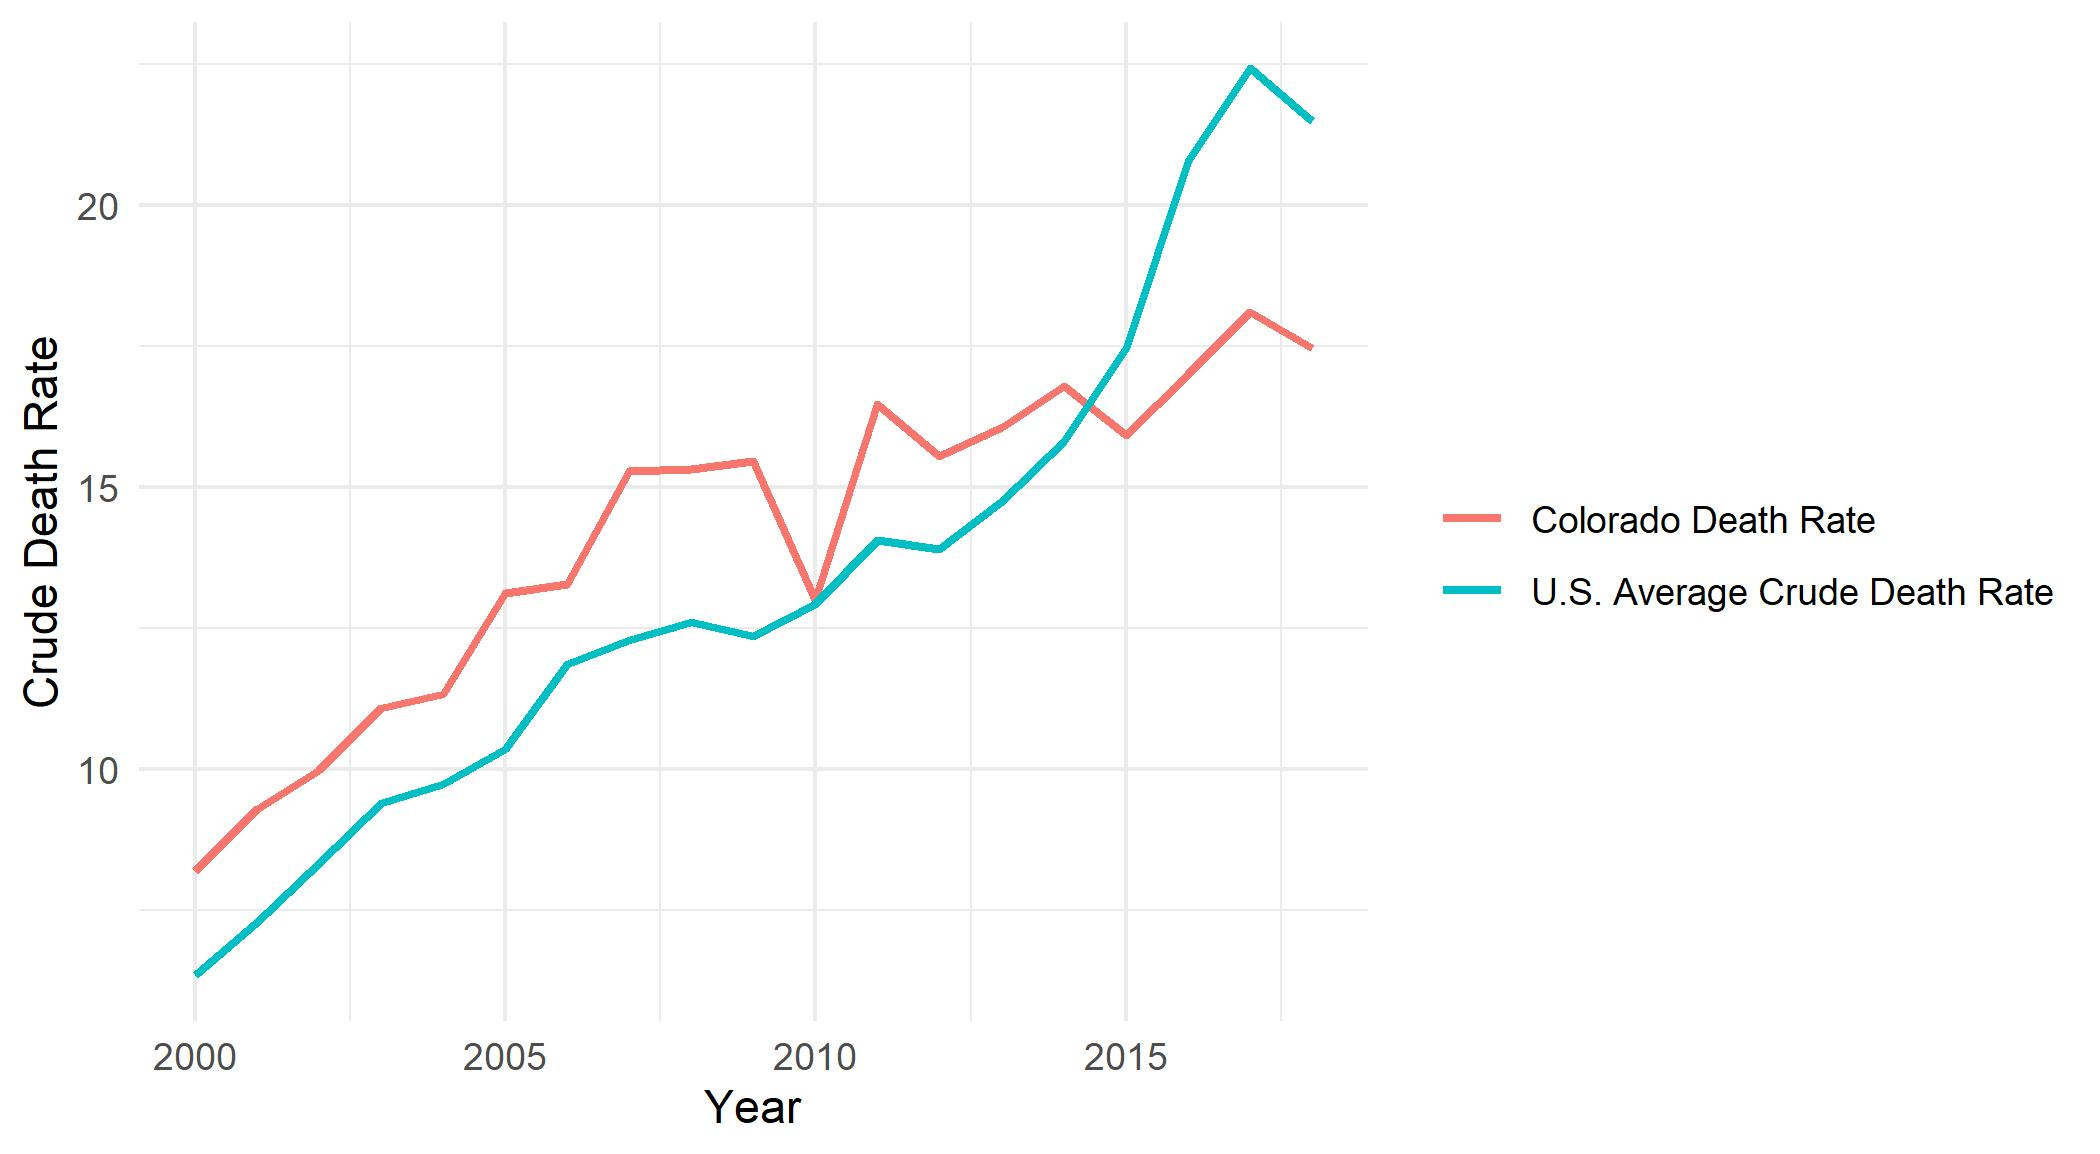
\includegraphics[width=0.85\textwidth]{death_rates_trend}
	\end{center}
	\caption{Drug Poisoning Death Rates Trend (2000-2018)}
	\label{fig:death_rates_trend}
\end{figure}

This paper seeks to estimate the causal effect of cannabis legalization on drug poisoning deaths in Colorado. We aim to do this by using synthetic control, a quasi-experimental research design, to examine the changes in the crude death rate for drug poisoning deaths in Colorado vs. states that have not legalized. 

\section{Data}

The data employed for this paper originates from two sources. First, we source data on drug poisoning deaths, population, and an estimate of the crude drug poisoning death rate from the United States Center for Disease Control (``CDC''). Second, we source state-level demographic data from IPUMS USA, which is a database harmonizing, organizing, and structuring data from various population surveys in the United States over time.

The first data set contains summary statistics by state and by year from 1999 to 2018. For each state in each year, the data reports the number of deaths due to drug poisoning, the population, and the ratio of the two previous variables as the crude death rate. Additionally, this data reports an estimate of the standard error for the crude death rate, and a lower and upper confidence interval around the point estimate. In addition to these base estimates, the data originally includes age-adjusted rates with standard errors and confidence intervals and the United State-wide crude death rate and United State-wide age-adjusted death rate. 

From this data set, we focus on the crude death rate for the state and extract this variable along with the state and year variables for data merging purposes. We focus our attention on the crude death rate statistic for a couple of important reasons. First, using the death rate as opposed to the total number of deaths allows us to immediately control for differences in state population when estimating our model. Second, we exclude the age-adjusted rate because our model also accounts for age demographics explicitly as covariates, so it would be inappropriate to use this as our outcome variable of interest.

The second data set contains nearly 28 million entries where each entry represents a person included in [[a survey]] in a particular year.  Importantly, this data includes the year and state in which that entry resided along with extensive demographic data. Thus, we are able to use the groups of these entries associated with each year and each state and calculate demographic summary information representative of each year in each state. We include in our demographic summaries the proportion of the population that is listed as male as compared to female [[should footnote simplicity of coding here ( I don't remember seeing info about non-binary or choose not to identify)]], a summary of a few significant age buckets, proportions of the population based on race, on marital status, on education, and on employment status. Additionally, we summarize the mean number of hours worked, the median income, the mean number of children, and the mean number of children under 5 years old. We present the mean and standard deviation of each of these demographic variables in Table \ref{tab:var_summary}.

To construct our final data set for use in analysis, we combine the two data sources. Since we have summarized the latter data set at the state and year level and the first data set is already at this level, we merge on the state and year. Thus, we have data for each state, inclusive of Washington D.C., for each year between 2000 and 2018 with data on deaths associated with drug poisoning, population, crude death rate, and all of our descriptive demographics data.

\begin{table}[H]

\caption{\label{tab:tab:var_summary}Variable Summary}
\centering
\begin{tabular}[t]{lrr}
\toprule
Variable & Mean & Std. Dev\\
\midrule
\addlinespace[0.3em]
\multicolumn{3}{l}{\textbf{Drug Poisonings}}\\
\hspace{1em}\cellcolor{gray!6}{Deaths} & \cellcolor{gray!6}{777.179} & \cellcolor{gray!6}{887.743}\\
\hspace{1em}Population & 5995451.840 & 6730237.227\\
\hspace{1em}\cellcolor{gray!6}{Crude Death Rate} & \cellcolor{gray!6}{13.381} & \cellcolor{gray!6}{7.082}\\
\addlinespace[0.3em]
\multicolumn{3}{l}{\textbf{Gender Population Proportions}}\\
\hspace{1em}Male & 0.489 & 0.012\\
\hspace{1em}\cellcolor{gray!6}{Female} & \cellcolor{gray!6}{0.511} & \cellcolor{gray!6}{0.012}\\
\addlinespace[0.3em]
\multicolumn{3}{l}{\textbf{Age Population Proportions}}\\
\hspace{1em}Under 30 & 0.176 & 0.022\\
\hspace{1em}\cellcolor{gray!6}{Under 50} & \cellcolor{gray!6}{0.450} & \cellcolor{gray!6}{0.042}\\
\hspace{1em}Over 50 & 0.374 & 0.045\\
\addlinespace[0.3em]
\multicolumn{3}{l}{\textbf{Race Population Proportions}}\\
\hspace{1em}\cellcolor{gray!6}{American Indian} & \cellcolor{gray!6}{0.018} & \cellcolor{gray!6}{0.039}\\
\hspace{1em}Asian & 0.039 & 0.070\\
\hspace{1em}\cellcolor{gray!6}{Black} & \cellcolor{gray!6}{0.088} & \cellcolor{gray!6}{0.094}\\
\hspace{1em}Other Race & 0.045 & 0.039\\
\hspace{1em}\cellcolor{gray!6}{White} & \cellcolor{gray!6}{0.810} & \cellcolor{gray!6}{0.131}\\
\addlinespace[0.3em]
\multicolumn{3}{l}{\textbf{Marital Status Population Proportions}}\\
\hspace{1em}Married & 0.609 & 0.062\\
\hspace{1em}\cellcolor{gray!6}{Not Married} & \cellcolor{gray!6}{0.391} & \cellcolor{gray!6}{0.062}\\
\addlinespace[0.3em]
\multicolumn{3}{l}{\textbf{Education Population Proportions}}\\
\hspace{1em}Less High School & 0.084 & 0.029\\
\hspace{1em}\cellcolor{gray!6}{High School} & \cellcolor{gray!6}{0.372} & \cellcolor{gray!6}{0.050}\\
\hspace{1em}Some College & 0.247 & 0.036\\
\hspace{1em}\cellcolor{gray!6}{College} & \cellcolor{gray!6}{0.191} & \cellcolor{gray!6}{0.034}\\
\hspace{1em}Higher College & 0.106 & 0.041\\
\addlinespace[0.3em]
\multicolumn{3}{l}{\textbf{Employment Population Proportions and Summary Statistics}}\\
\hspace{1em}\cellcolor{gray!6}{Employed} & \cellcolor{gray!6}{0.724} & \cellcolor{gray!6}{0.045}\\
\hspace{1em}Not Employed & 0.276 & 0.045\\
\hspace{1em}\cellcolor{gray!6}{Mean Hrs Worked} & \cellcolor{gray!6}{32.222} & \cellcolor{gray!6}{2.269}\\
\hspace{1em}Median Income & 22380.650 & 5043.007\\
\addlinespace[0.3em]
\multicolumn{3}{l}{\textbf{Children Summary Statistics}}\\
\hspace{1em}\cellcolor{gray!6}{Mean Children} & \cellcolor{gray!6}{0.823} & \cellcolor{gray!6}{0.107}\\
\hspace{1em}Mean Children Under 5 years old & 0.168 & 0.029\\
\bottomrule
\end{tabular}
\end{table}


\section{Methodology}

We utilize the synthetic control method first developed by Abadie and Gardeazabal (2003) and then expanded upon in Abadie et. al (2010)(2015). Similar to Abadie et. al (2010) we are analyzing the impact of a government policy shock. In this analysis we are estimating the impact of Colorado's legalization of recreation cannabis in 2012. For our synthetic control, Colorado is the treatment state of interest, and we have a donor pool of 41[Need to double check that's correct] states. The synthetic control method [MORE INFO HERE]

Suppose that we have $1,2...S+1$ states and let $s = 1$ be the treated state, additionally we have $t = 1,2...T$ time periods where $T_0$ represents the number of pretreatment periods, and $T_0 + 1...T$ are the posttreatment periods. With that let $Y_{st}$ be the crude death rate for state $s$ at time $t$. In a posttreatment time line we are estimating
\begin{equation*}
\hat{\alpha} = Y_{1t} - \sum_{s=2}^{S+1}w^{*}Y_{st}
\end{equation*}
$w^{*}_s$ is a vector of optimally chosen weights for states from our donor pool to represent our synthetic Colorado. Again deriving from Abadie (2010) $w^{*}_s$ is the vector of weights that minimizes the following equation
\begin{equation*}
(X_1 - X_0w)'V(X_1 - X_0w)
\end{equation*}
$X_1$ is a $(K \times 1)$ vector of state population variables and $X_0$ is a $(K \times S)$ matrix of state population variables for $S$ donor states. Note that $w_s \geq 0$ and $\sum w_s = 1$.

We utilize the weights generated to create a synthetic Colorado, where we examine the counterfactual of a Colorado that never legalized recreational cannabis. Additionally we follow Abadie (2010) and use their placebo technique as a robustness check. The placebo technique consists of assigning each state in our donor pool as the treated state and then creating an optimal $w^{*}_s$, from the other donor states as well as the treated state, in the pretreatment period. Utilizing the weights we calculate the posttreatment root mean squared prediction error (RMSPE) for each state. We then take a ratio between the post/pretreatment RMSPE for each state. We expect this value to be high for our treated state, which would suggest that the posttreatment RMSPE is large due to the differences between the synthetic and the observed Colorado.

\section{Results}

\subsection{Model}

By applying the techniques described above, we are able to construct a synthetic Colorado with weights on the donor states such that the synthetic Colorado's crude death rate closely matches actual Colorado''s crude death rate in the period preceding legalization of recreational marijuana. Table \ref{tab:unit_weight_table_colorado} displays the weights for each of the donor states with a contribution to Synthetic Colorado over 0.1 percent. We see that Arizona and New Hampshire contribute most significantly to Synthetic Colorado, with weights of approximately 45 and 38 percent, respectively. We also see Washington D.C. (District of Columbia) and Utah contributing at a health level of approximately 10 and 8 percent, respectively. Though many donor states have nonzero weights in our analysis, we exclude them from this table because they contribute at a level below 0.1 percent.

\begin{table}[H]

\caption{\label{tab:unit_weight_table_colorado}Synthetic Weights}
\centering
\begin{tabular}[t]{lr}
\toprule
Unit & Weight\\
\midrule
\cellcolor{gray!6}{Alabama} & \cellcolor{gray!6}{0.0000000}\\
Arizona & 0.4537880\\
\cellcolor{gray!6}{Arkansas} & \cellcolor{gray!6}{0.0000000}\\
Connecticut & 0.0000016\\
\cellcolor{gray!6}{Delaware} & \cellcolor{gray!6}{0.0000000}\\
\addlinespace
District of Columbia & 0.0946779\\
\cellcolor{gray!6}{Florida} & \cellcolor{gray!6}{0.0000000}\\
Georgia & 0.0000000\\
\cellcolor{gray!6}{Hawaii} & \cellcolor{gray!6}{0.0000001}\\
Idaho & 0.0000000\\
\addlinespace
\cellcolor{gray!6}{Illinois} & \cellcolor{gray!6}{0.0000000}\\
Indiana & 0.0000000\\
\cellcolor{gray!6}{Iowa} & \cellcolor{gray!6}{0.0000000}\\
Kansas & 0.0000001\\
\cellcolor{gray!6}{Kentucky} & \cellcolor{gray!6}{0.0000000}\\
\addlinespace
Louisiana & 0.0000000\\
\cellcolor{gray!6}{Maryland} & \cellcolor{gray!6}{0.0000000}\\
Minnesota & 0.0000603\\
\cellcolor{gray!6}{Mississippi} & \cellcolor{gray!6}{0.0000000}\\
Missouri & 0.0000000\\
\addlinespace
\cellcolor{gray!6}{Montana} & \cellcolor{gray!6}{0.0000000}\\
Nebraska & 0.0000001\\
\cellcolor{gray!6}{New Hampshire} & \cellcolor{gray!6}{0.3754123}\\
New Jersey & 0.0000001\\
\cellcolor{gray!6}{New Mexico} & \cellcolor{gray!6}{0.0000000}\\
\addlinespace
New York & 0.0000000\\
\cellcolor{gray!6}{North Carolina} & \cellcolor{gray!6}{0.0000000}\\
North Dakota & 0.0000005\\
\cellcolor{gray!6}{Ohio} & \cellcolor{gray!6}{0.0000000}\\
Oklahoma & 0.0000000\\
\addlinespace
\cellcolor{gray!6}{Pennsylvania} & \cellcolor{gray!6}{0.0000000}\\
Rhode Island & 0.0000000\\
\cellcolor{gray!6}{South Carolina} & \cellcolor{gray!6}{0.0000000}\\
South Dakota & 0.0000000\\
\cellcolor{gray!6}{Tennessee} & \cellcolor{gray!6}{0.0000000}\\
\addlinespace
Texas & 0.0000005\\
\cellcolor{gray!6}{Utah} & \cellcolor{gray!6}{0.0760580}\\
Virginia & 0.0000001\\
\cellcolor{gray!6}{West Virginia} & \cellcolor{gray!6}{0.0000000}\\
Wisconsin & 0.0000000\\
\addlinespace
\cellcolor{gray!6}{Wyoming} & \cellcolor{gray!6}{0.0000000}\\
\bottomrule
\end{tabular}
\end{table}


Next, we present the aggregate level predictors used in the model and compare them across Colorado, Synthetic Colorado, and the overall donor sample. We note that there are some differences between the observed Colorado and our synthetic Colorado, specifically regarding education level. However, the synthetic Colorado provides a much better estimation of the observed Colorado than our donor pool. 

\begin{table}[H]

\caption{\label{tab:balance_table_colorado}Balance Table}
\centering
\begin{tabular}[t]{lrrr}
\toprule
Variable & Colorado & Synthetic Colorado & Donor Sample\\
\midrule
\cellcolor{gray!6}{American Indian Proportion} & \cellcolor{gray!6}{0.009} & \cellcolor{gray!6}{0.022} & \cellcolor{gray!6}{0.014}\\
Asian Proportion & 0.026 & 0.025 & 0.035\\
\cellcolor{gray!6}{Black Proportion} & \cellcolor{gray!6}{0.030} & \cellcolor{gray!6}{0.059} & \cellcolor{gray!6}{0.098}\\
College Proportion & 0.245 & 0.204 & 0.184\\
\cellcolor{gray!6}{Employed Proportion} & \cellcolor{gray!6}{0.753} & \cellcolor{gray!6}{0.732} & \cellcolor{gray!6}{0.726}\\
\addlinespace
Female Proportion & 0.508 & 0.514 & 0.515\\
\cellcolor{gray!6}{Hispanic Proportion} & \cellcolor{gray!6}{0.139} & \cellcolor{gray!6}{0.120} & \cellcolor{gray!6}{0.067}\\
High School Proportion & 0.304 & 0.341 & 0.384\\
\cellcolor{gray!6}{Less Than High School Proportion} & \cellcolor{gray!6}{0.068} & \cellcolor{gray!6}{0.084} & \cellcolor{gray!6}{0.090}\\
Male Proportion & 0.492 & 0.486 & 0.485\\
\addlinespace
\cellcolor{gray!6}{Married Proportion} & \cellcolor{gray!6}{0.632} & \cellcolor{gray!6}{0.604} & \cellcolor{gray!6}{0.627}\\
Mean Children & 0.813 & 0.848 & 0.844\\
\cellcolor{gray!6}{Mean Children U5} & \cellcolor{gray!6}{0.183} & \cellcolor{gray!6}{0.179} & \cellcolor{gray!6}{0.174}\\
Mean Hrs Worked & 33.882 & 32.677 & 32.706\\
\cellcolor{gray!6}{Median Income} & \cellcolor{gray!6}{24523.077} & \cellcolor{gray!6}{23473.869} & \cellcolor{gray!6}{21327.955}\\
\addlinespace
More Than College Proportion & 0.130 & 0.122 & 0.100\\
\cellcolor{gray!6}{Not Employed Proportion} & \cellcolor{gray!6}{0.247} & \cellcolor{gray!6}{0.268} & \cellcolor{gray!6}{0.274}\\
Not Hispanic Proportion & 0.861 & 0.880 & 0.933\\
\cellcolor{gray!6}{Not Married Proportion} & \cellcolor{gray!6}{0.368} & \cellcolor{gray!6}{0.396} & \cellcolor{gray!6}{0.373}\\
Other Race Proportion & 0.064 & 0.056 & 0.041\\
\addlinespace
\cellcolor{gray!6}{Over 50 Proportion} & \cellcolor{gray!6}{0.337} & \cellcolor{gray!6}{0.348} & \cellcolor{gray!6}{0.360}\\
Some College Proportion & 0.253 & 0.250 & 0.242\\
\cellcolor{gray!6}{Under 30 Proportion} & \cellcolor{gray!6}{0.180} & \cellcolor{gray!6}{0.180} & \cellcolor{gray!6}{0.175}\\
Under 50 Proportion & 0.483 & 0.472 & 0.466\\
\cellcolor{gray!6}{White Proportion} & \cellcolor{gray!6}{0.870} & \cellcolor{gray!6}{0.837} & \cellcolor{gray!6}{0.813}\\
\bottomrule
\end{tabular}
\end{table}


\subsection{Estimated Impact}

We now plot the observed Colorado versus our synthetic Colorado in Figure \ref{fig:trends_plot_colorado} below. The dashed vertical line indicates when treatment begins. As we noted above our synthetic Colorado is very similar to the observed Colorado, which we see below. In the pre-treatment period our synthetic Colorado tracks closely with the observed Colorado. In the post-treatment period, we see the sharp separation from the synthetic and the observed. 

\begin{figure}[H]
	\begin{center}
		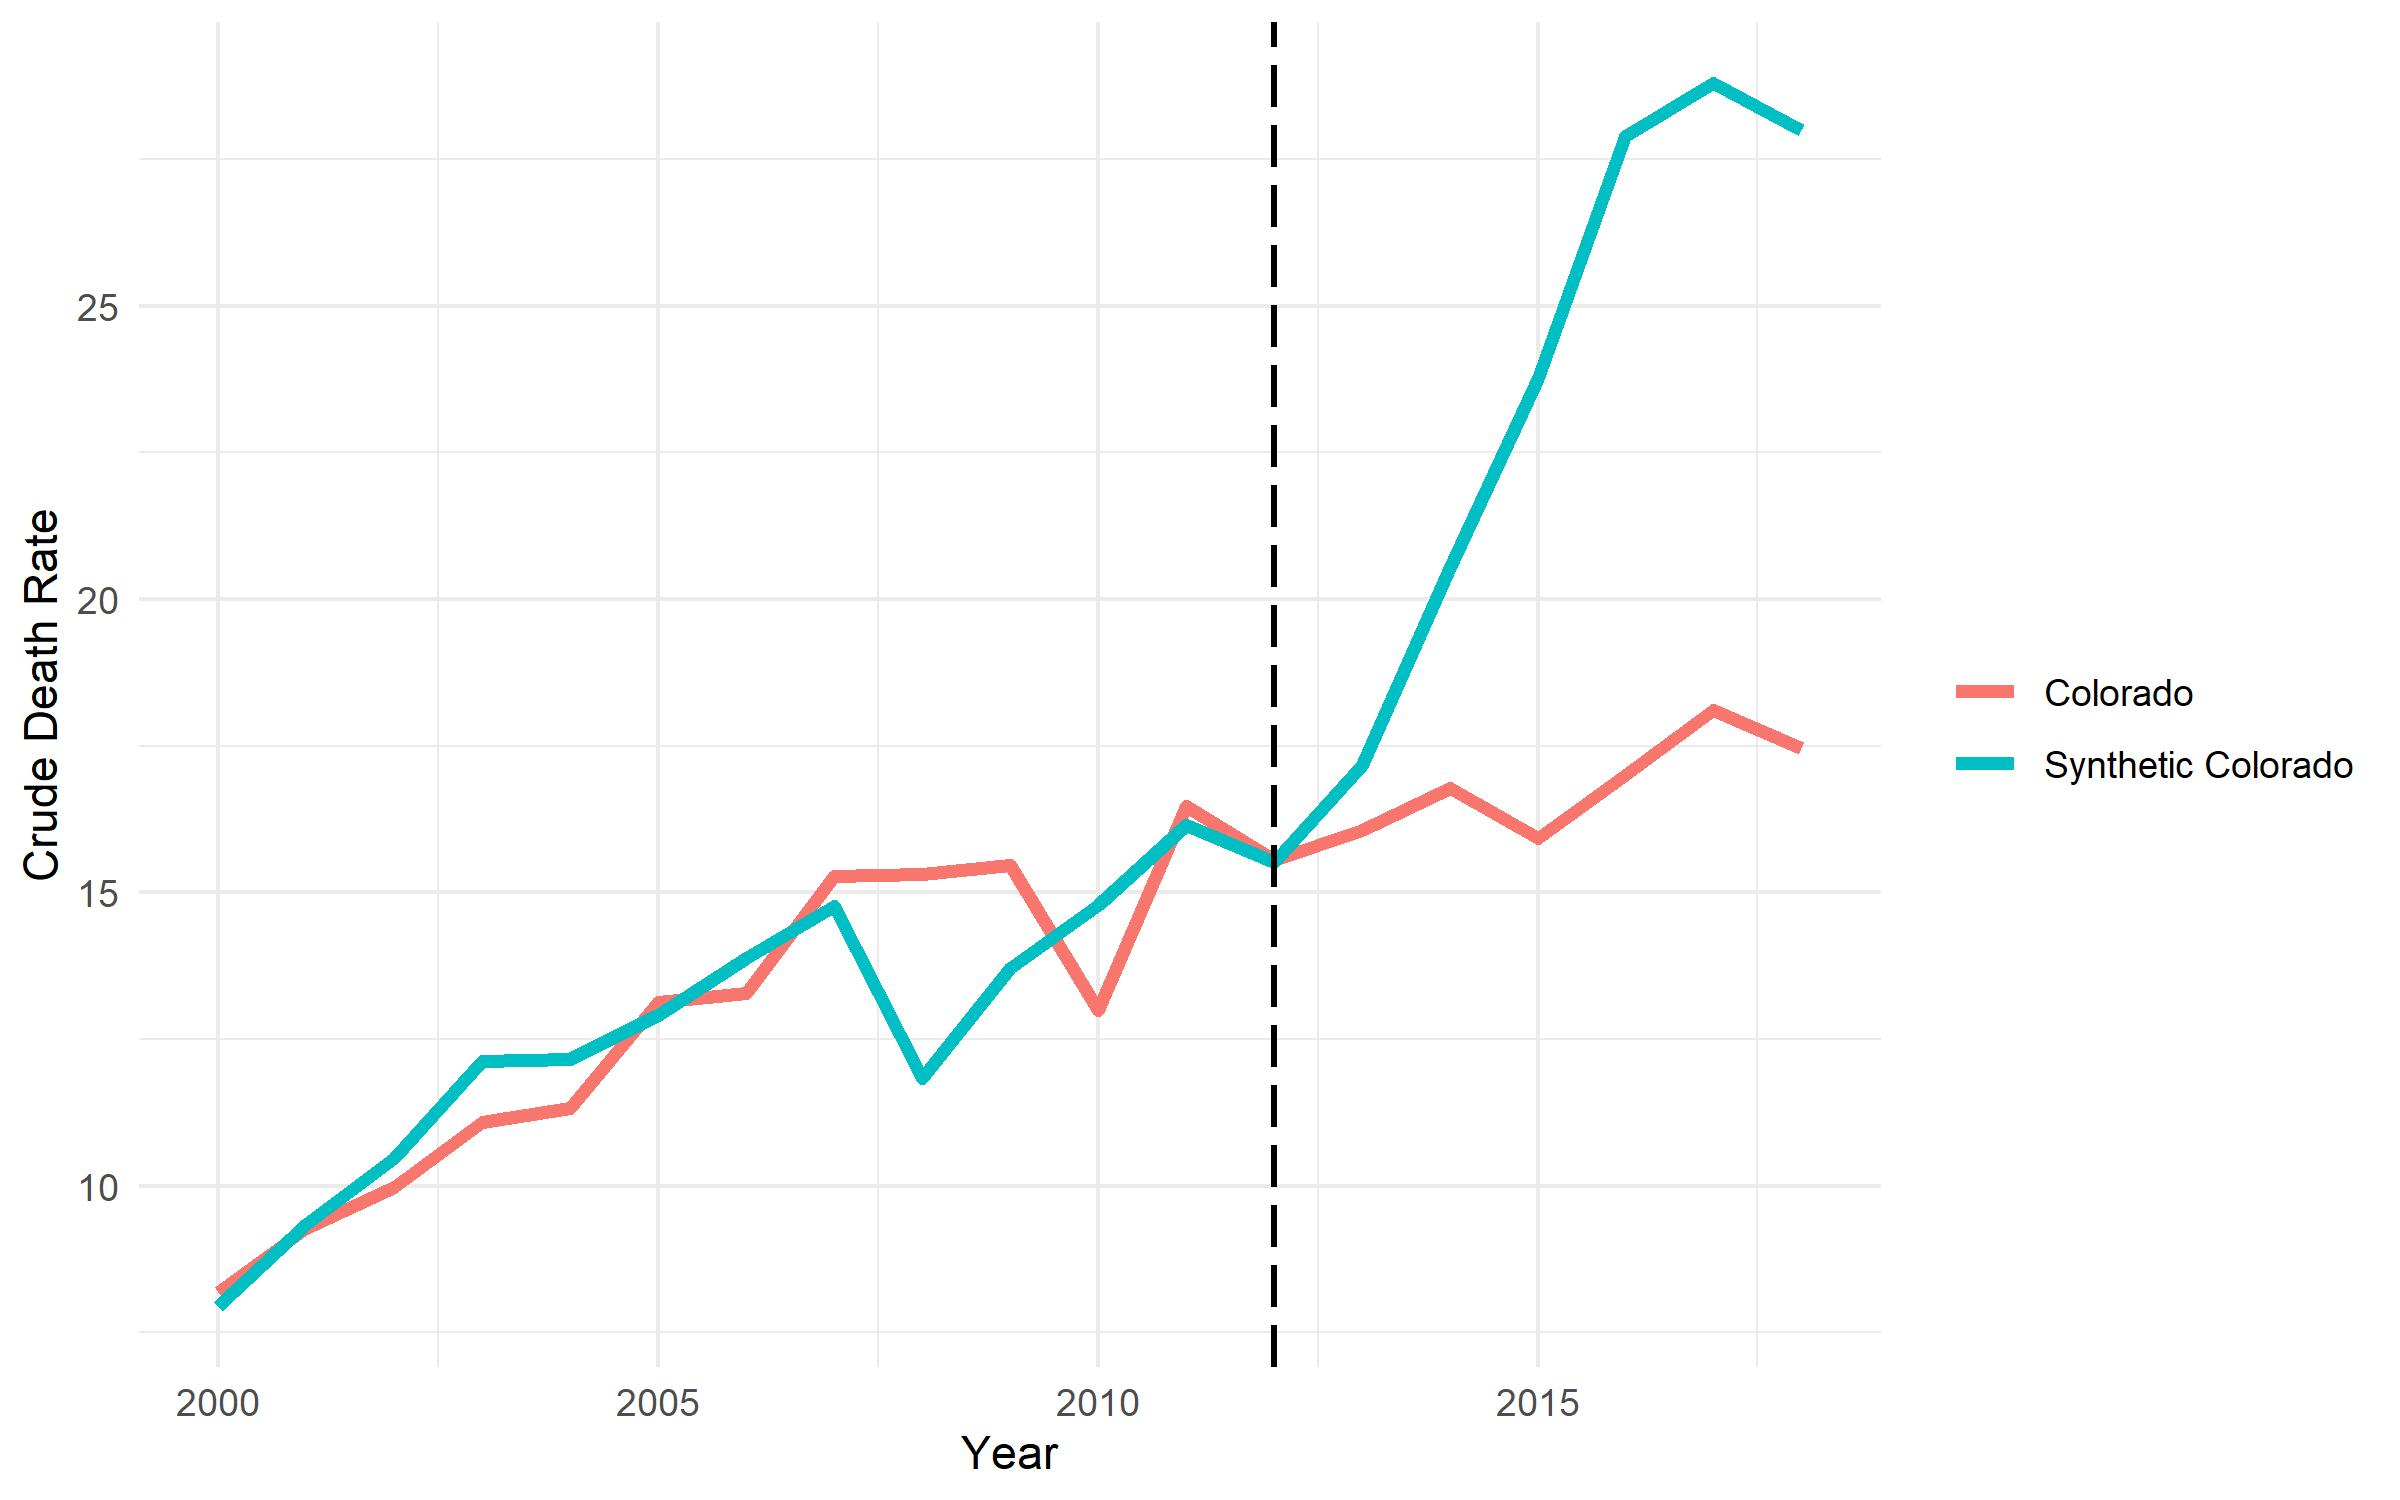
\includegraphics[width=0.85\textwidth]{trends_plot_colorado}
	\end{center}
	\caption{Trends in Crude Death Rate: Colorado vs. Synthetic Colorado}
	\label{fig:trends_plot_colorado}
\end{figure}

In Figure \ref{fig:diffs_plot_colorado} we plot the gap between the synthetic and observed.

\begin{figure}[H]
	\begin{center}
		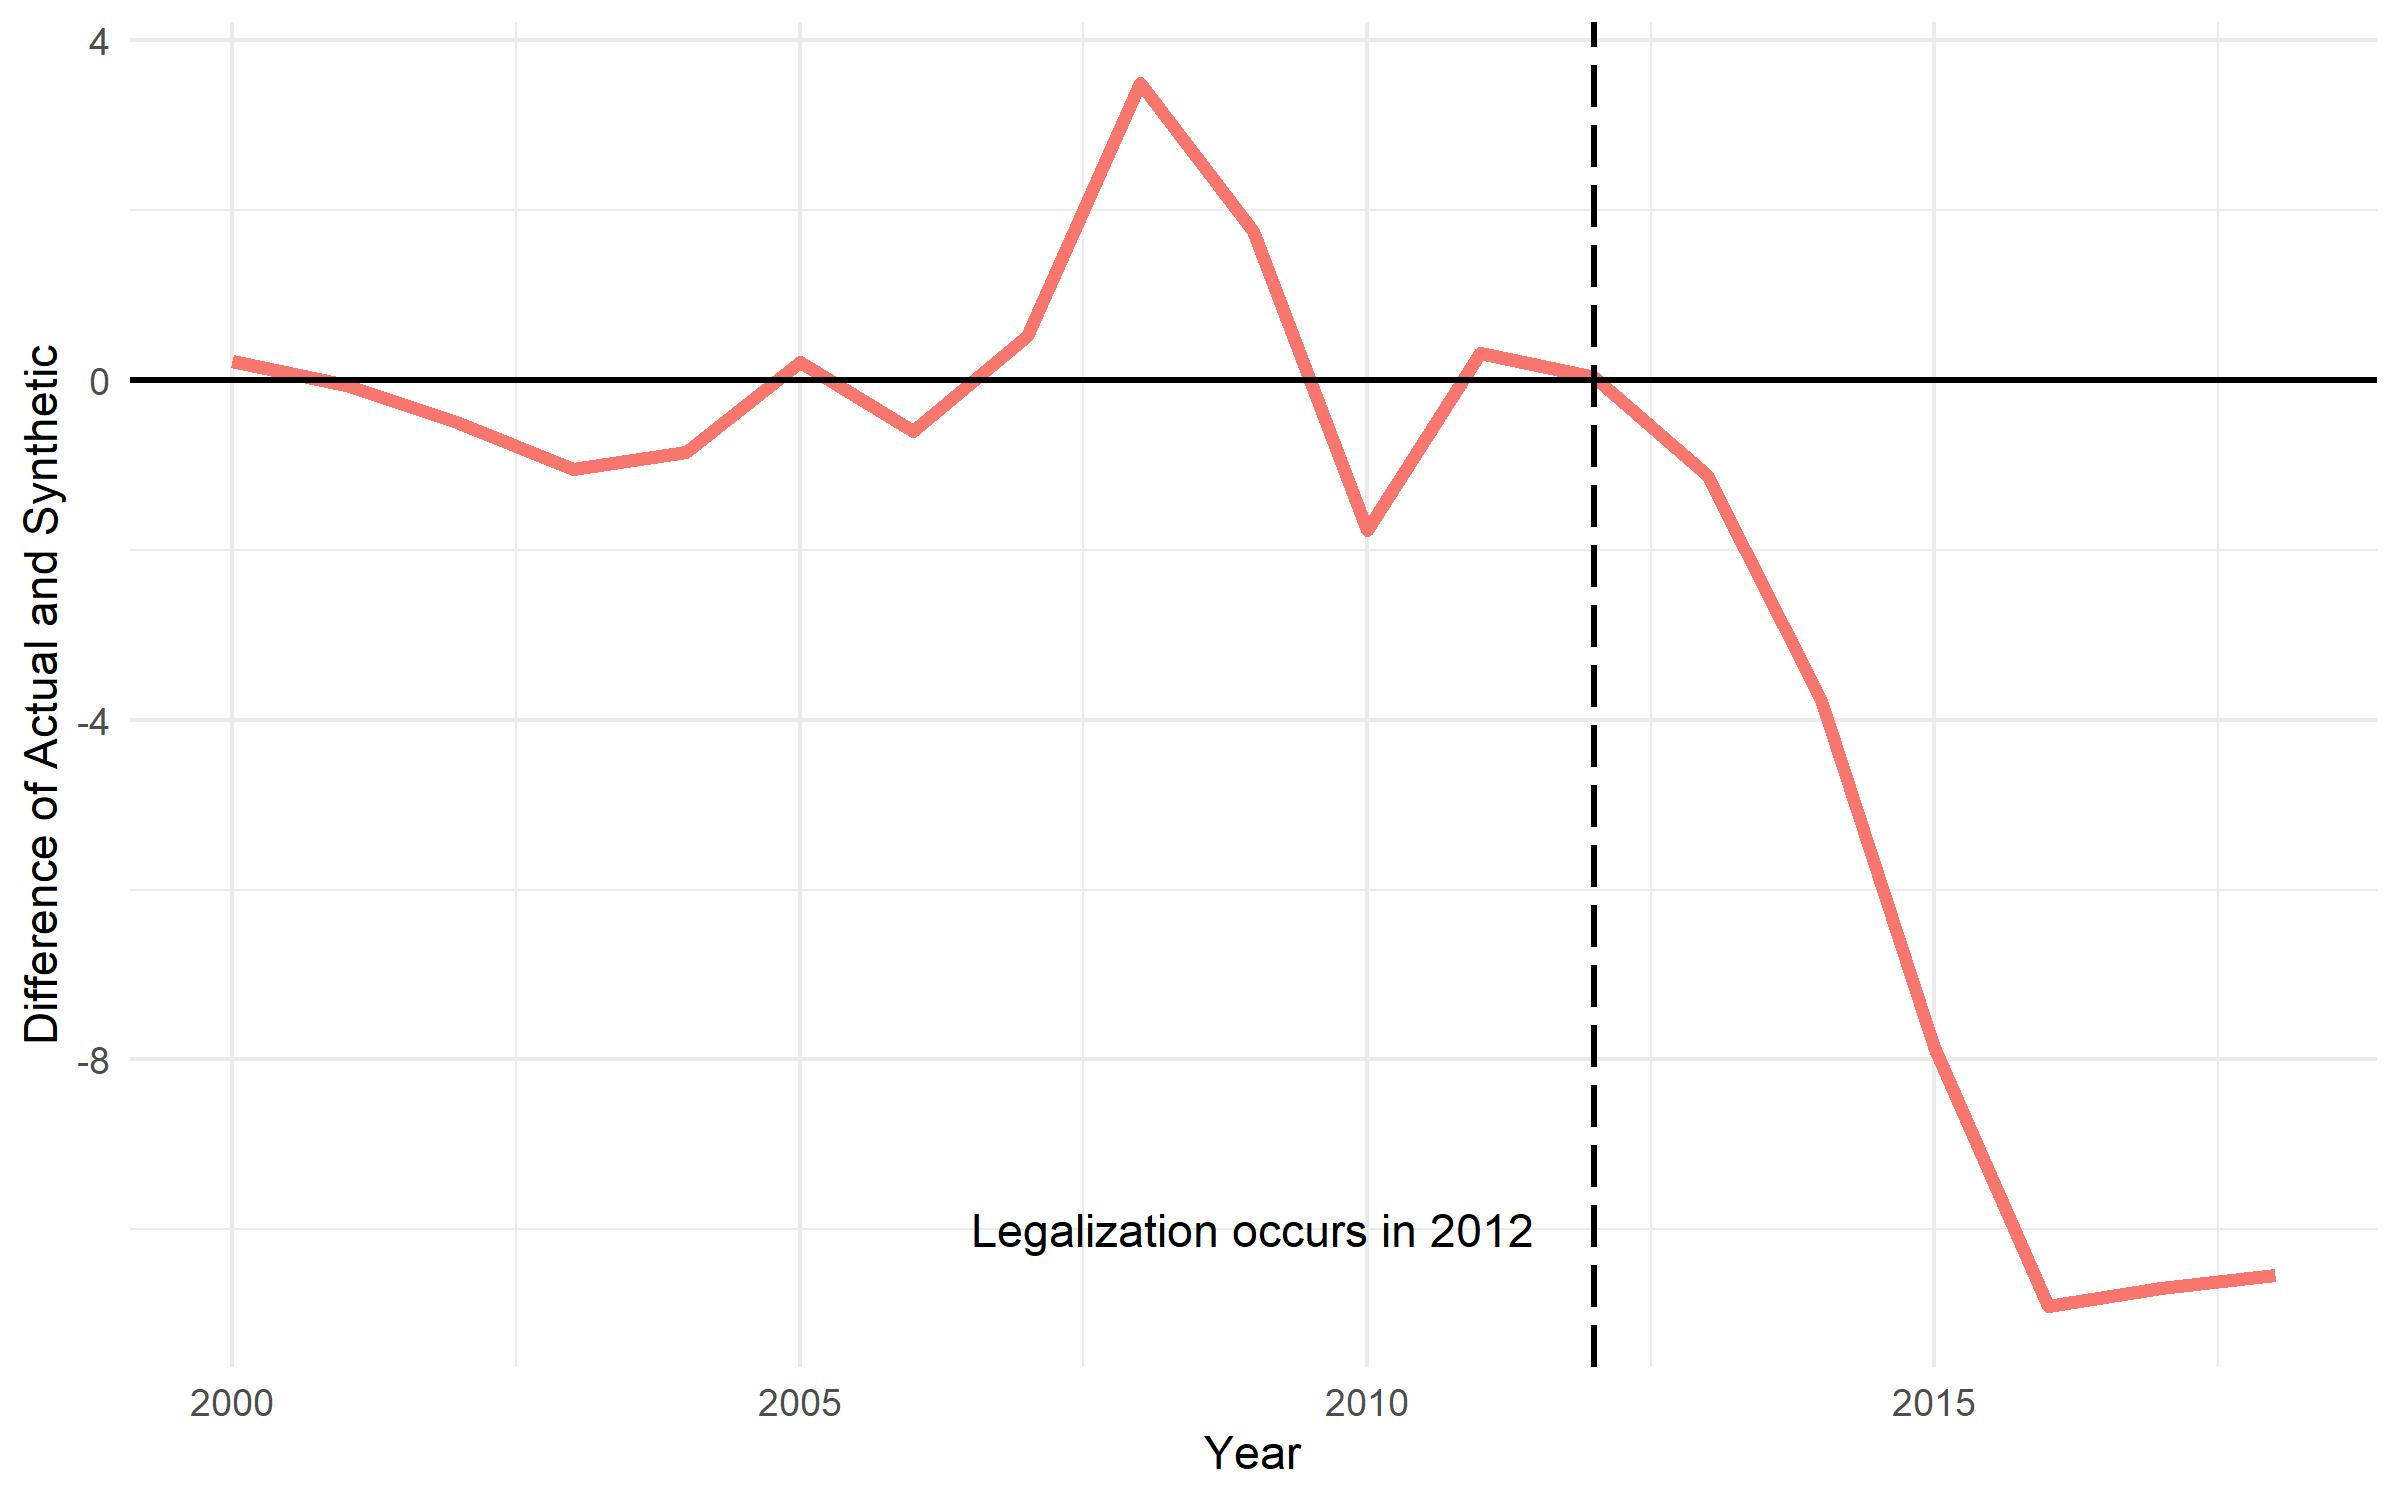
\includegraphics[width=0.85\textwidth]{diffs_plot_colorado}
	\end{center}
	\caption{Differences in Crude Death Rate}
	\label{fig:diffs_plot_colorado}
\end{figure}

Finally, we present the numerical results associated with Figure \ref{fig:diffs_plot_colorado} in \ref{tab:causal_est_table_colorado}. We estimate the causal effect of legalization of Marijuana on crude death rate in Colorado to be a decline of approximately 3.75 two years after legalization, decline of approximately 10.9 four years after legalization, and a decline of approximately 10.5 six years after legalization.

\begin{table}[H]

\caption{\label{tab:causal_est_table_colorado}Estimated Impact of Legalization on Death Rate: Colorado}
\centering
\begin{tabular}[t]{rrrr}
\toprule
Years After Legalization & Real Death Rate & Synthetic Death Rate & Estimated Causal Effect\\
\midrule
\cellcolor{gray!6}{2} & \cellcolor{gray!6}{16.785} & \cellcolor{gray!6}{20.552} & \cellcolor{gray!6}{-3.767}\\
4 & 17.002 & 27.899 & -10.897\\
\cellcolor{gray!6}{6} & \cellcolor{gray!6}{17.470} & \cellcolor{gray!6}{28.002} & \cellcolor{gray!6}{-10.532}\\
\bottomrule
\end{tabular}
\end{table}


\subsection{Robustness Checks}

In Figure \ref{fig:mspe_plot_colorado} below we plot the ratio between the post-treatment MSPE and the pre-treatment MSPE. What we expect to see is that the treated unit will have a small pre-treatment MSPE which would indicate a close fit between the observed and synthetic units in the pre-treatment period. We would also expect to see the post-treatment MSPE to be large as that would indicate a separation between the observed and synthetic units. We see that generally holds in the figure below, with Colorado standing well differentiated from each other state with the exception of New Hampshire. [[Need to explain New Hampshire - I think we ought to ask Cunningham. I don't know how to explain this]]

\begin{figure}[H]
	\begin{center}
		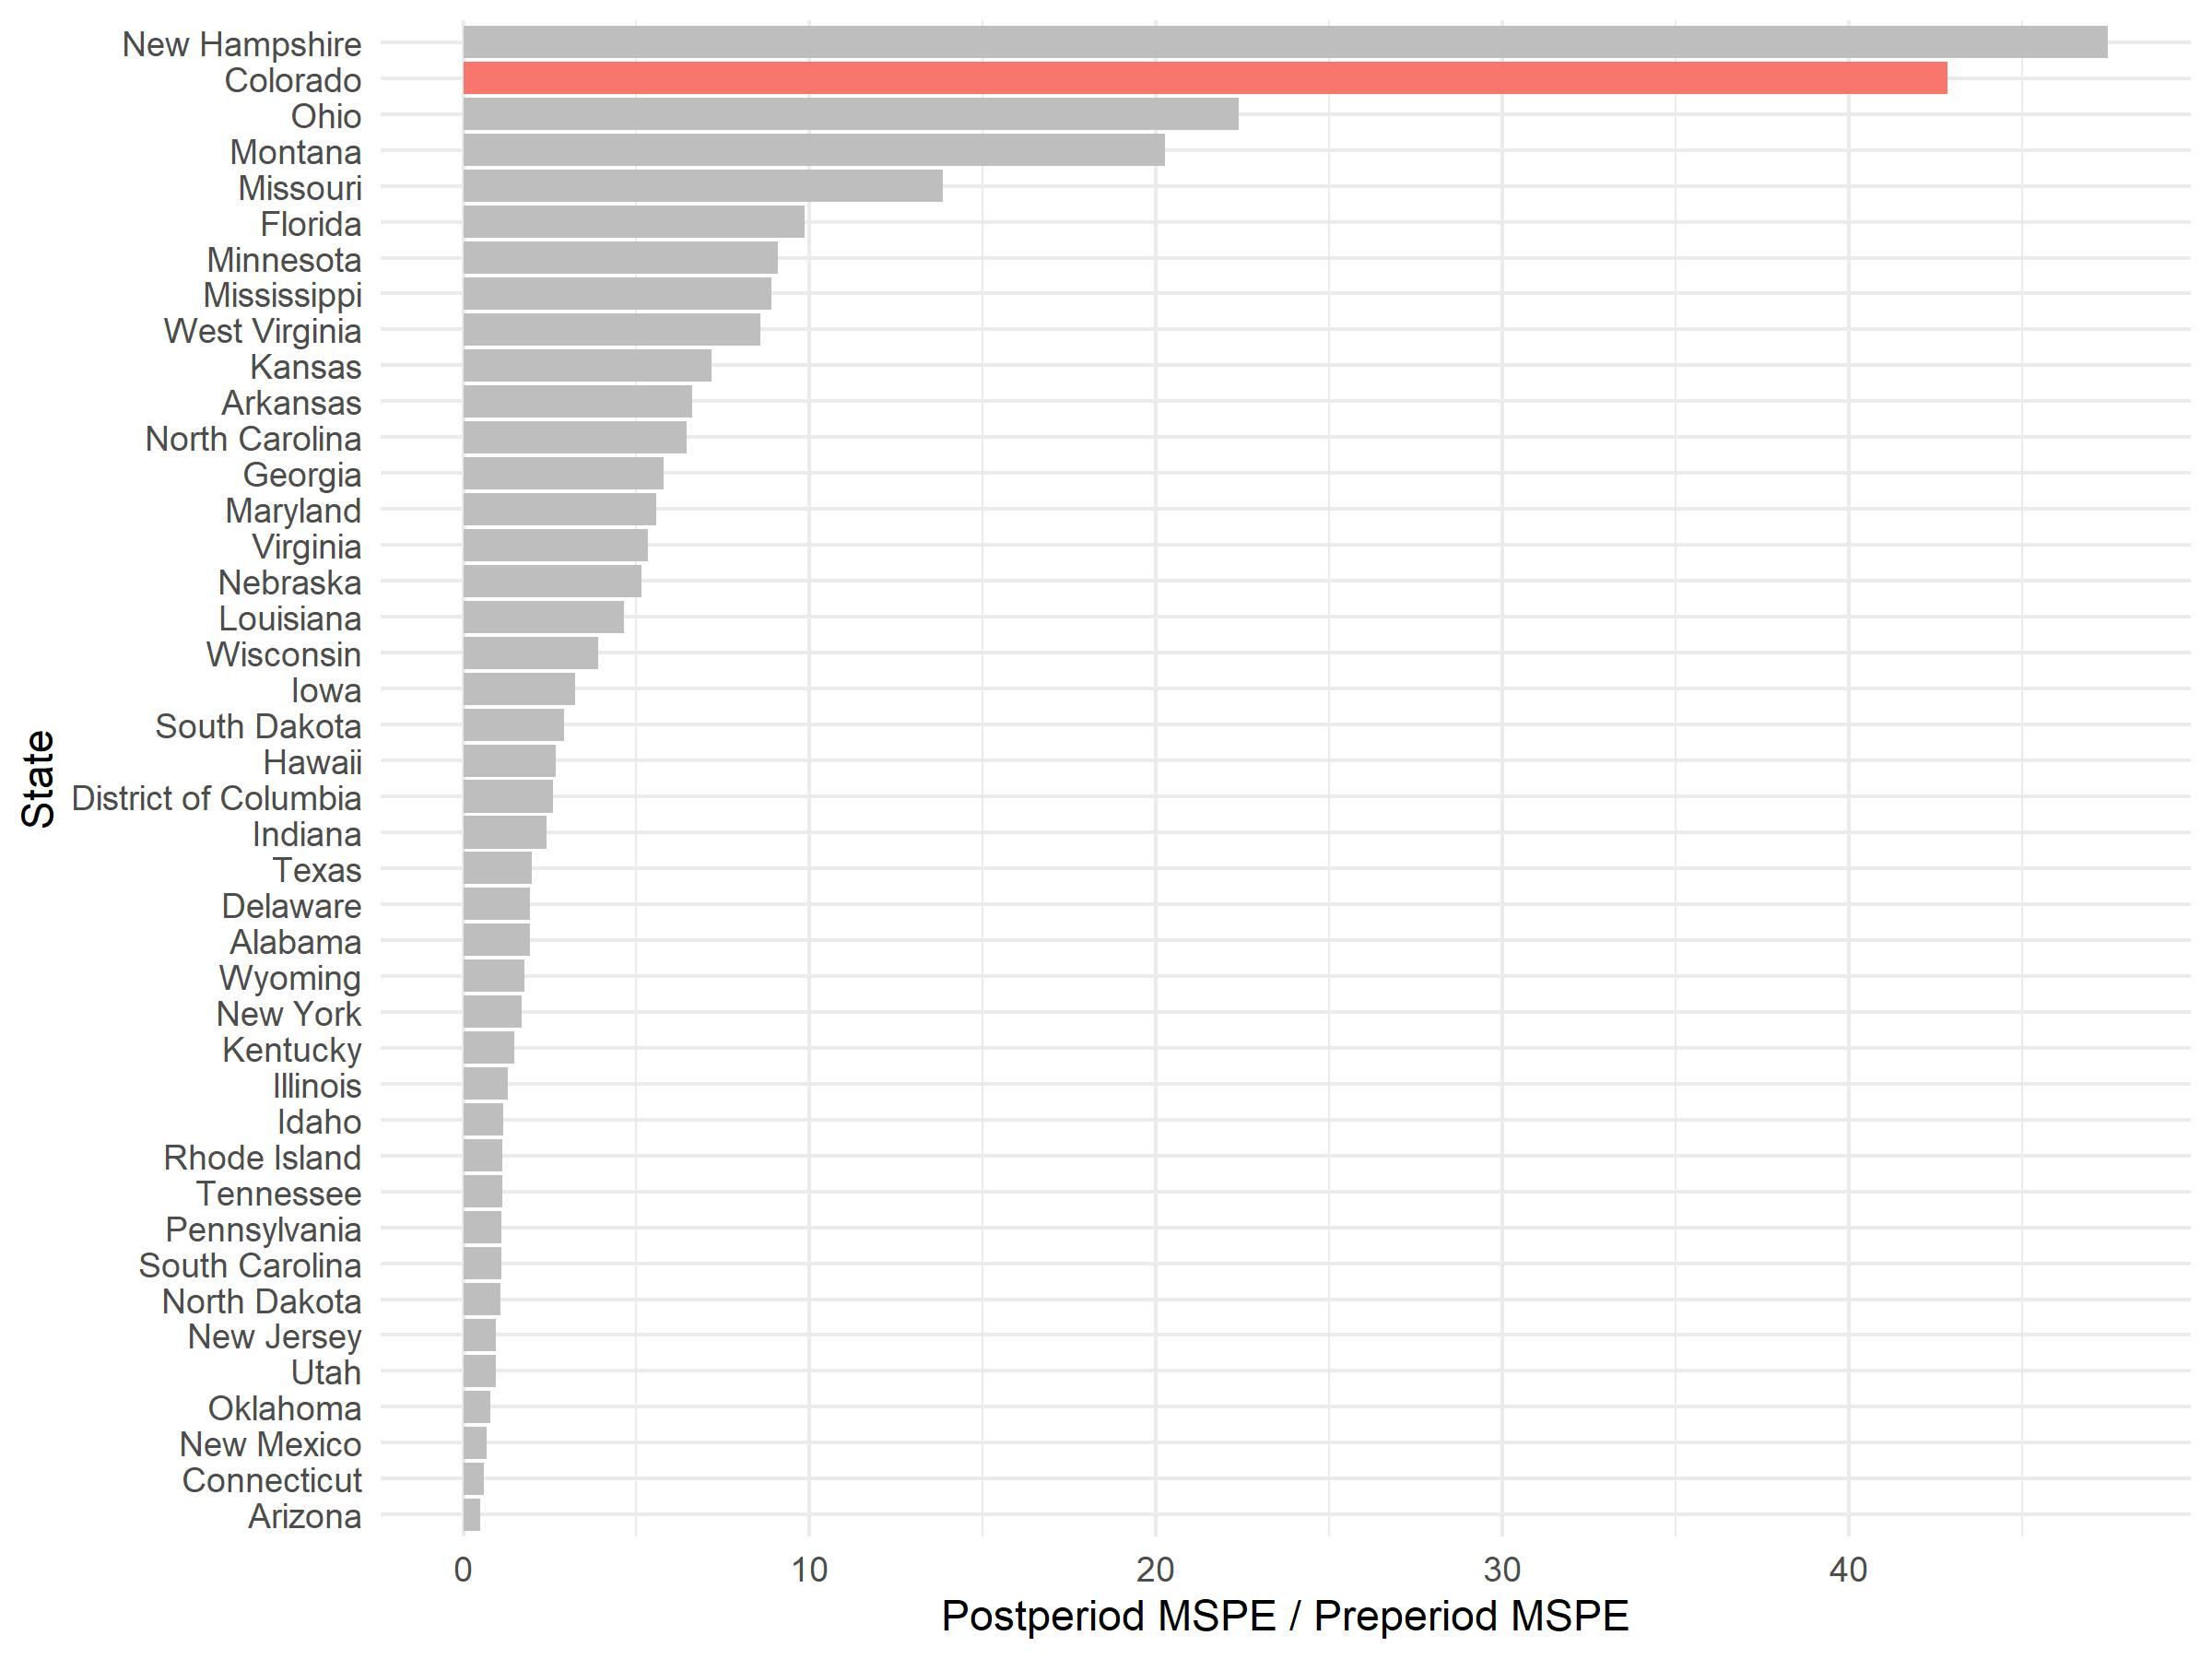
\includegraphics[width=0.85\textwidth]{mspe_plot_colorado}
	\end{center}
	\caption{MSPE Ratio Plot}
	\label{fig:mspe_plot_colorado}
\end{figure}

As a robustness check we perform the placebo test as suggested by Abadie et al. (2010). When performing the placebo, we reassign the treatment to each state in the donor pool while placing Colorado into the donor pool. We then run synthetic control on all the donor states and plot their outcomes in Figure \ref{fig:placebos_plot_colorado} below.

\begin{figure}[H]
	\begin{center}
		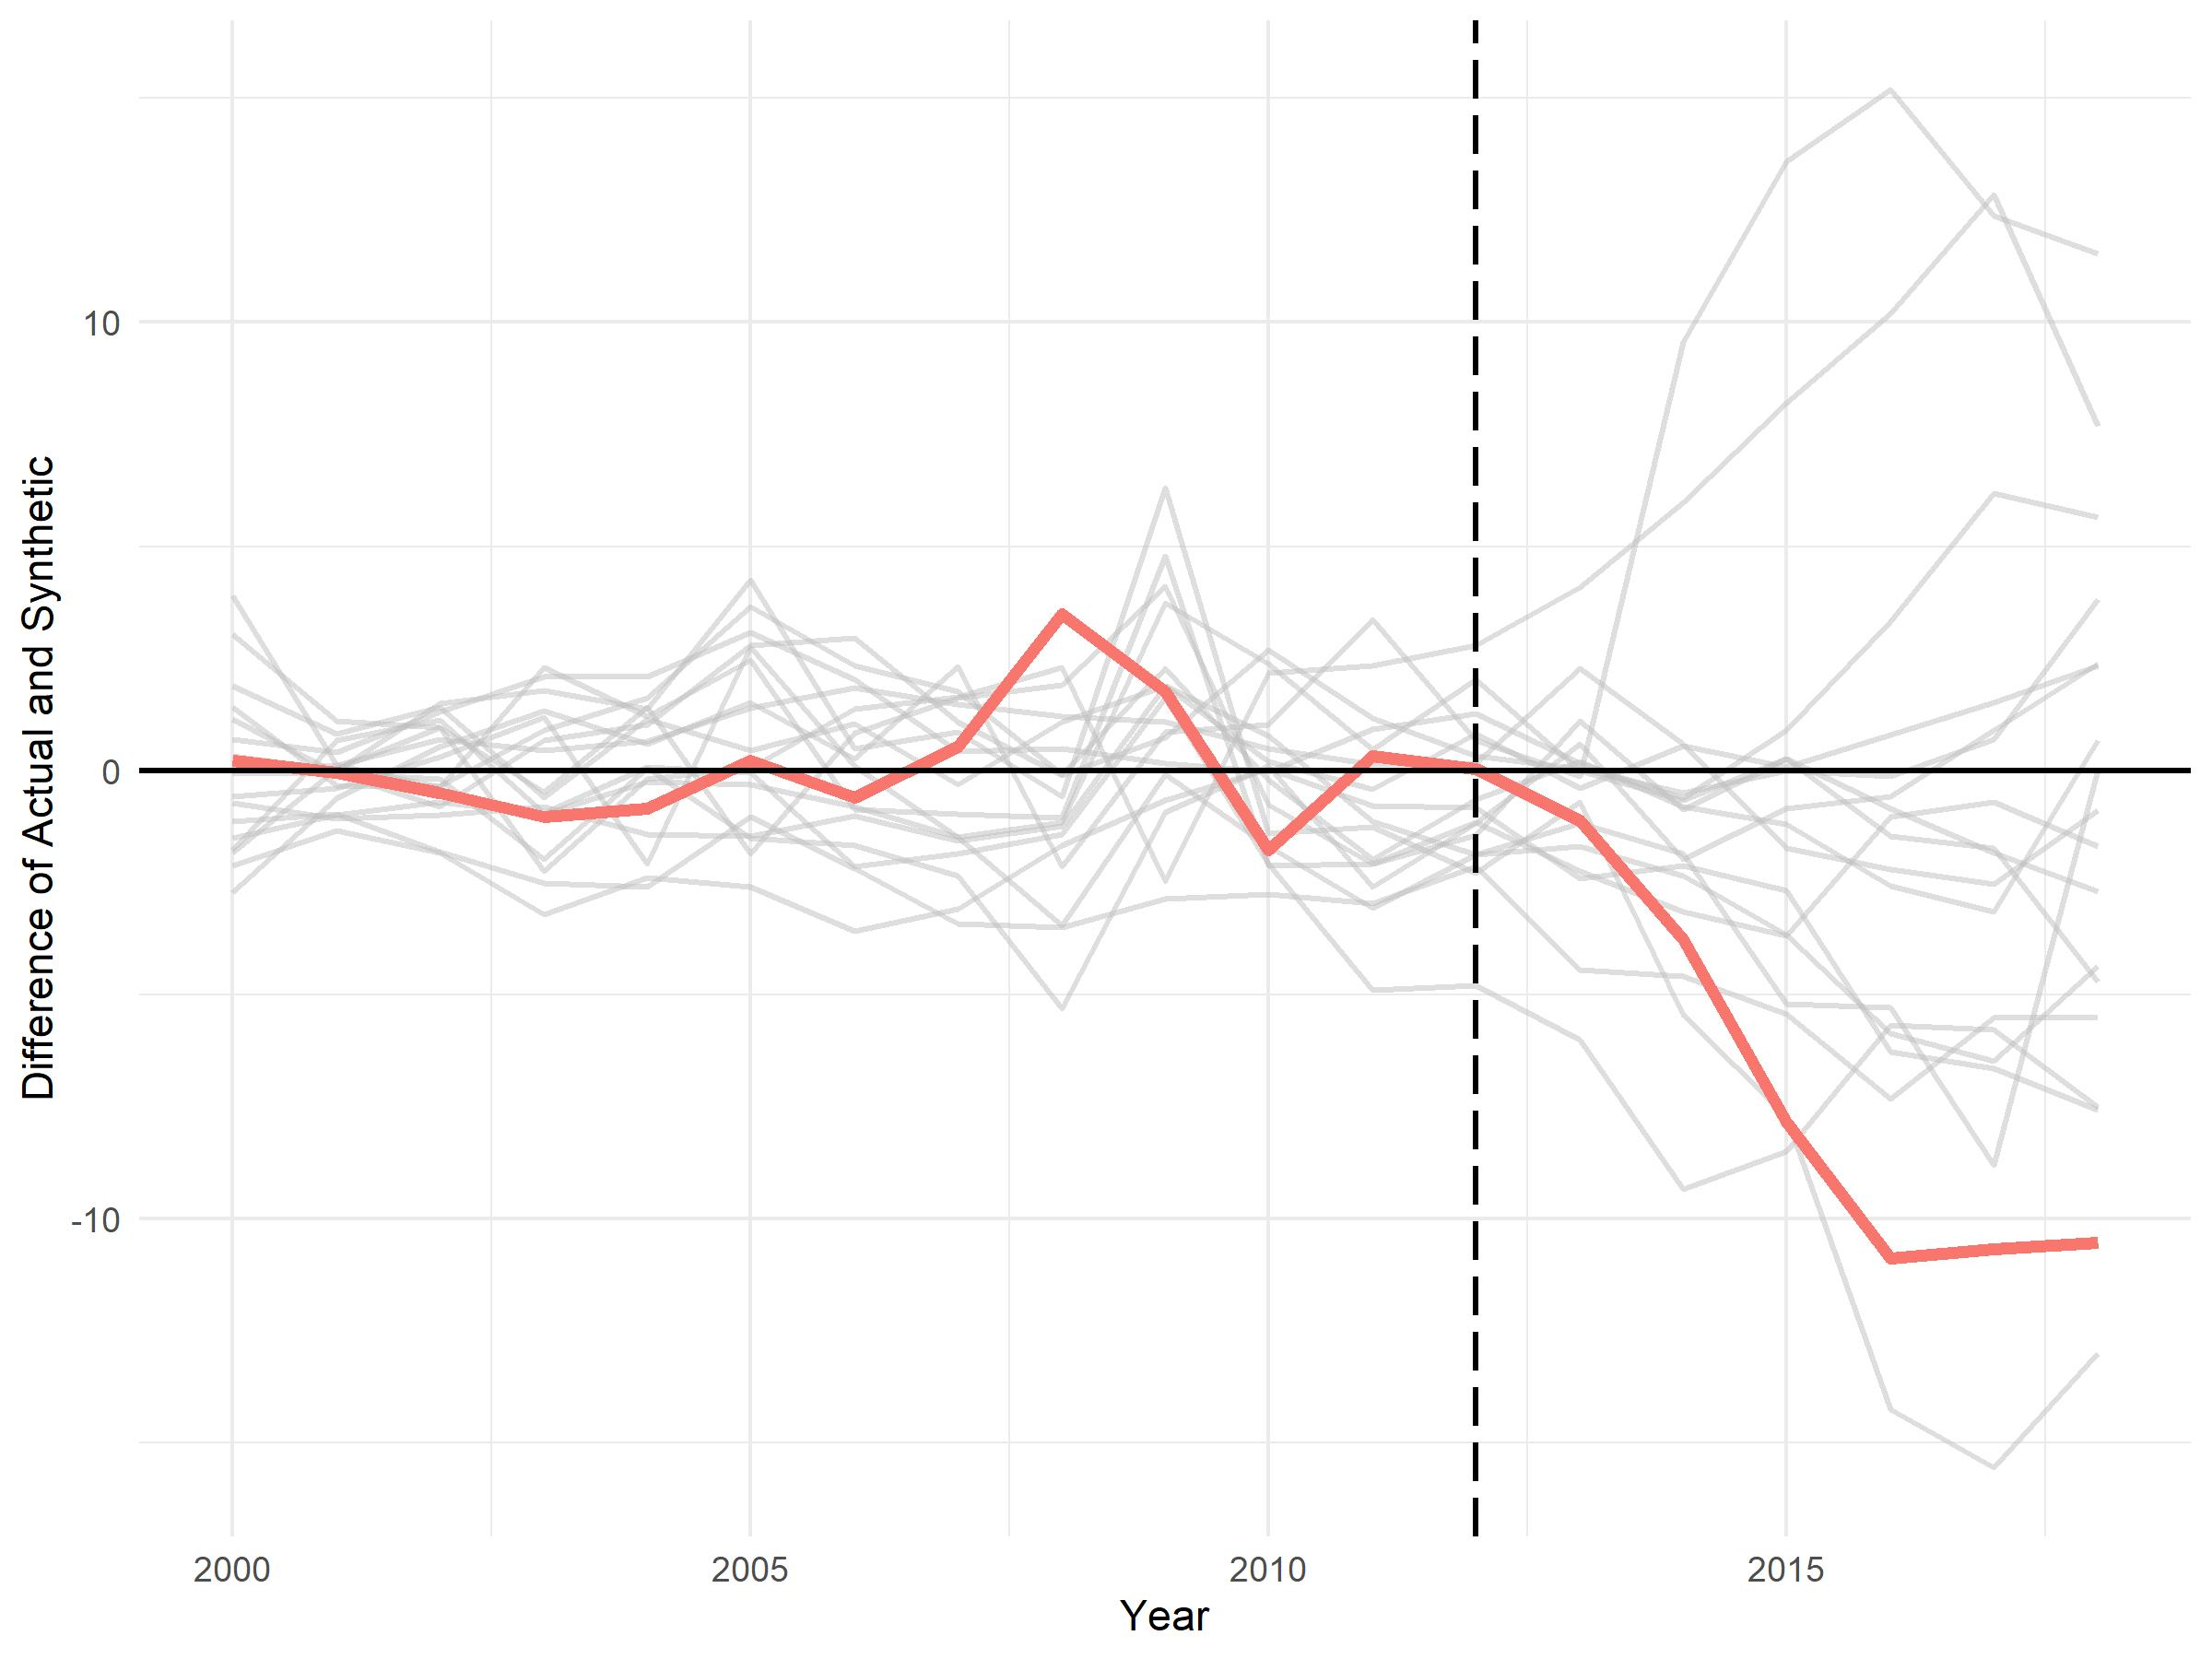
\includegraphics[width=0.85\textwidth]{placebos_plot_colorado}
	\end{center}
	\caption{Placebos Plot}
	\label{fig:placebos_plot_colorado}
\end{figure}

To ensure we are comparing our result for Colorado with comparably fit placebos, we only chart and assess placebos for which their pretreatment period RMSPE is less than or equal to double the Colorado pretreatment period RMSPE. This is because we are interested in assessing models where the fit is relatively good in the pretreatment period, not those that we were not able to fit in the pretreatment period. As shown in the figure above, the placebo test confirms the strength of our results, with only one placebo falling below Colorado.  Montana ... [[Explain why?]]

For our final robustness check, we apply the same methodology described here and above to another state, Washington, that legalized marijuana at the same time as Colorado (2012). We present detailed results of this analysis in the appendix. When applying our synthetic control model to Washington, we find similarly statistically significant results, albeit with less sizable estimated causal effects. We estimate a decline in crude death rate of 2.3 two years removed from treatment, 6.4 four years after treatment, and 6.4 again six years after treatment.

\section{Discussion}

Our findings in this paper strongly support the notion that legalization of marijuana has \emph{some} positive societal benefit. Entirely separate from the potential economic gains of a new high growth industry and the job and tax revenue creation that implies, we have shown that there are potential social benefits. Perhaps it is not the case that marijuana is simply a gateway drug - perhaps it is rather the case that marijuana can provide a more gentle release than other intoxicating substitutes, and actually decrease drug risk overall. Our finding of a non negligible decrease in drug poisoning death rate in both Colorado and Washington in years following legalization of recreational marijuana use supports this notion, and potentially supports legalization more broadly across the United States.

We recognize that an interesting limit on the general applicability of our results is the heterogeneity of states and regions in the United States, and that broadly applying a legalization policy may not have identical positive effects. State and regional preferences, attitudes, and political leanings often impact how these sort of policies are received and can drastically change usage outcomes. It is worth noting that Colorado and Washington both are historically known as states that are more friendly and curious regarding recreational use of drugs, which may skew results relative to a generally applied law. Nonetheless, our finding is logically supported by accessibility-driven decision making. Naturally, if something is more accessible, we're likely to reach for that instead as long as we view it as a viable substitute. If recreational marijuana is available and accessible, perhaps fewer people are going to the trouble of finding a black market drug supplier and acquiring harder, riskier drugs. Furthermore, the risk of death from overdosing on marijuana is nearly nonexistent, particularly when compared to other psychoactive drugs.

Additionally, we recognize that our findings carry some important limitations. One key limitation is in our data. We are only able to use data at the state and year level, reducing some of the granularity in our results. Furthermore, we are limited primarily to demographic data for this study, which  is limiting our the ability to fit our model. Though matching a synthetic state based on broad demographics is a good start, we would ideally expand our model predictors to provide more of a rich feature set. Ultimately, we are estimating drug poisoning death rate, so additional data relating to this outcome would be very useful in producing a richer and more accurate model. Another limitation is in the number of years of data we have to study. Though we have many years in the pretreatment period, we only have six years after treatment to assess impact. Ideally, we would have more years in the post-treatment period.

[[Patrick to write a paragraph here explaining the extensive method where you combine differential timing and synthetic control]]

\section{Appendix - Robustness check with Washington}



\begin{table}[H]

\caption{\label{tab:unit_weight_table_washington}Synthetic Weights}
\centering
\begin{tabular}[t]{lr}
\toprule
Unit & Weight\\
\midrule
\cellcolor{gray!6}{Florida} & \cellcolor{gray!6}{0.282}\\
Utah & 0.281\\
\cellcolor{gray!6}{Connecticut} & \cellcolor{gray!6}{0.212}\\
Montana & 0.115\\
\cellcolor{gray!6}{Hawaii} & \cellcolor{gray!6}{0.048}\\
\addlinespace
Arizona & 0.047\\
\cellcolor{gray!6}{District of Columbia} & \cellcolor{gray!6}{0.015}\\
\bottomrule
\multicolumn{2}{l}{\textsuperscript{a} Table excludes donor states}\\
\multicolumn{2}{l}{with 0.1 percent model}\\
\multicolumn{2}{l}{weight.}\\
\end{tabular}
\end{table}


\begin{table}[H]

\caption{\label{tab:balance_table_washington}Synthetic Washington Predictor Variable Balance Summary}
\centering
\begin{tabular}[t]{lrrr}
\toprule
Variable & Washington & Synthetic Washington & Donor Sample\\
\midrule
\cellcolor{gray!6}{American Indian Proportion} & \cellcolor{gray!6}{0.014} & \cellcolor{gray!6}{0.014} & \cellcolor{gray!6}{0.014}\\
Asian Proportion & 0.071 & 0.049 & 0.035\\
\cellcolor{gray!6}{Black Proportion} & \cellcolor{gray!6}{0.026} & \cellcolor{gray!6}{0.061} & \cellcolor{gray!6}{0.098}\\
College Proportion & 0.212 & 0.200 & 0.184\\
\cellcolor{gray!6}{Employed Proportion} & \cellcolor{gray!6}{0.719} & \cellcolor{gray!6}{0.728} & \cellcolor{gray!6}{0.726}\\
\addlinespace
Female Proportion & 0.510 & 0.513 & 0.515\\
\cellcolor{gray!6}{Hispanic Proportion} & \cellcolor{gray!6}{0.063} & \cellcolor{gray!6}{0.106} & \cellcolor{gray!6}{0.067}\\
High School Proportion & 0.332 & 0.356 & 0.384\\
\cellcolor{gray!6}{Less Than High School Proportion} & \cellcolor{gray!6}{0.065} & \cellcolor{gray!6}{0.072} & \cellcolor{gray!6}{0.090}\\
Male Proportion & 0.490 & 0.487 & 0.485\\
\addlinespace
\cellcolor{gray!6}{Married Proportion} & \cellcolor{gray!6}{0.626} & \cellcolor{gray!6}{0.638} & \cellcolor{gray!6}{0.627}\\
Mean Children & 0.817 & 0.935 & 0.844\\
\cellcolor{gray!6}{Mean Children U5} & \cellcolor{gray!6}{0.173} & \cellcolor{gray!6}{0.202} & \cellcolor{gray!6}{0.174}\\
Mean Hrs Worked & 31.858 & 32.302 & 32.706\\
\cellcolor{gray!6}{Median Income} & \cellcolor{gray!6}{22900.000} & \cellcolor{gray!6}{21956.634} & \cellcolor{gray!6}{21327.955}\\
\addlinespace
More Than College Proportion & 0.110 & 0.108 & 0.100\\
\cellcolor{gray!6}{Not Employed Proportion} & \cellcolor{gray!6}{0.281} & \cellcolor{gray!6}{0.272} & \cellcolor{gray!6}{0.274}\\
Not Hispanic Proportion & 0.937 & 0.894 & 0.933\\
\cellcolor{gray!6}{Not Married Proportion} & \cellcolor{gray!6}{0.374} & \cellcolor{gray!6}{0.362} & \cellcolor{gray!6}{0.373}\\
Other Race Proportion & 0.053 & 0.050 & 0.041\\
\addlinespace
\cellcolor{gray!6}{Over 50 Proportion} & \cellcolor{gray!6}{0.355} & \cellcolor{gray!6}{0.349} & \cellcolor{gray!6}{0.360}\\
Some College Proportion & 0.280 & 0.263 & 0.242\\
\cellcolor{gray!6}{Under 30 Proportion} & \cellcolor{gray!6}{0.173} & \cellcolor{gray!6}{0.186} & \cellcolor{gray!6}{0.175}\\
Under 50 Proportion & 0.472 & 0.466 & 0.466\\
\cellcolor{gray!6}{White Proportion} & \cellcolor{gray!6}{0.837} & \cellcolor{gray!6}{0.826} & \cellcolor{gray!6}{0.813}\\
\bottomrule
\end{tabular}
\end{table}


\begin{figure}[H]
	\begin{center}
		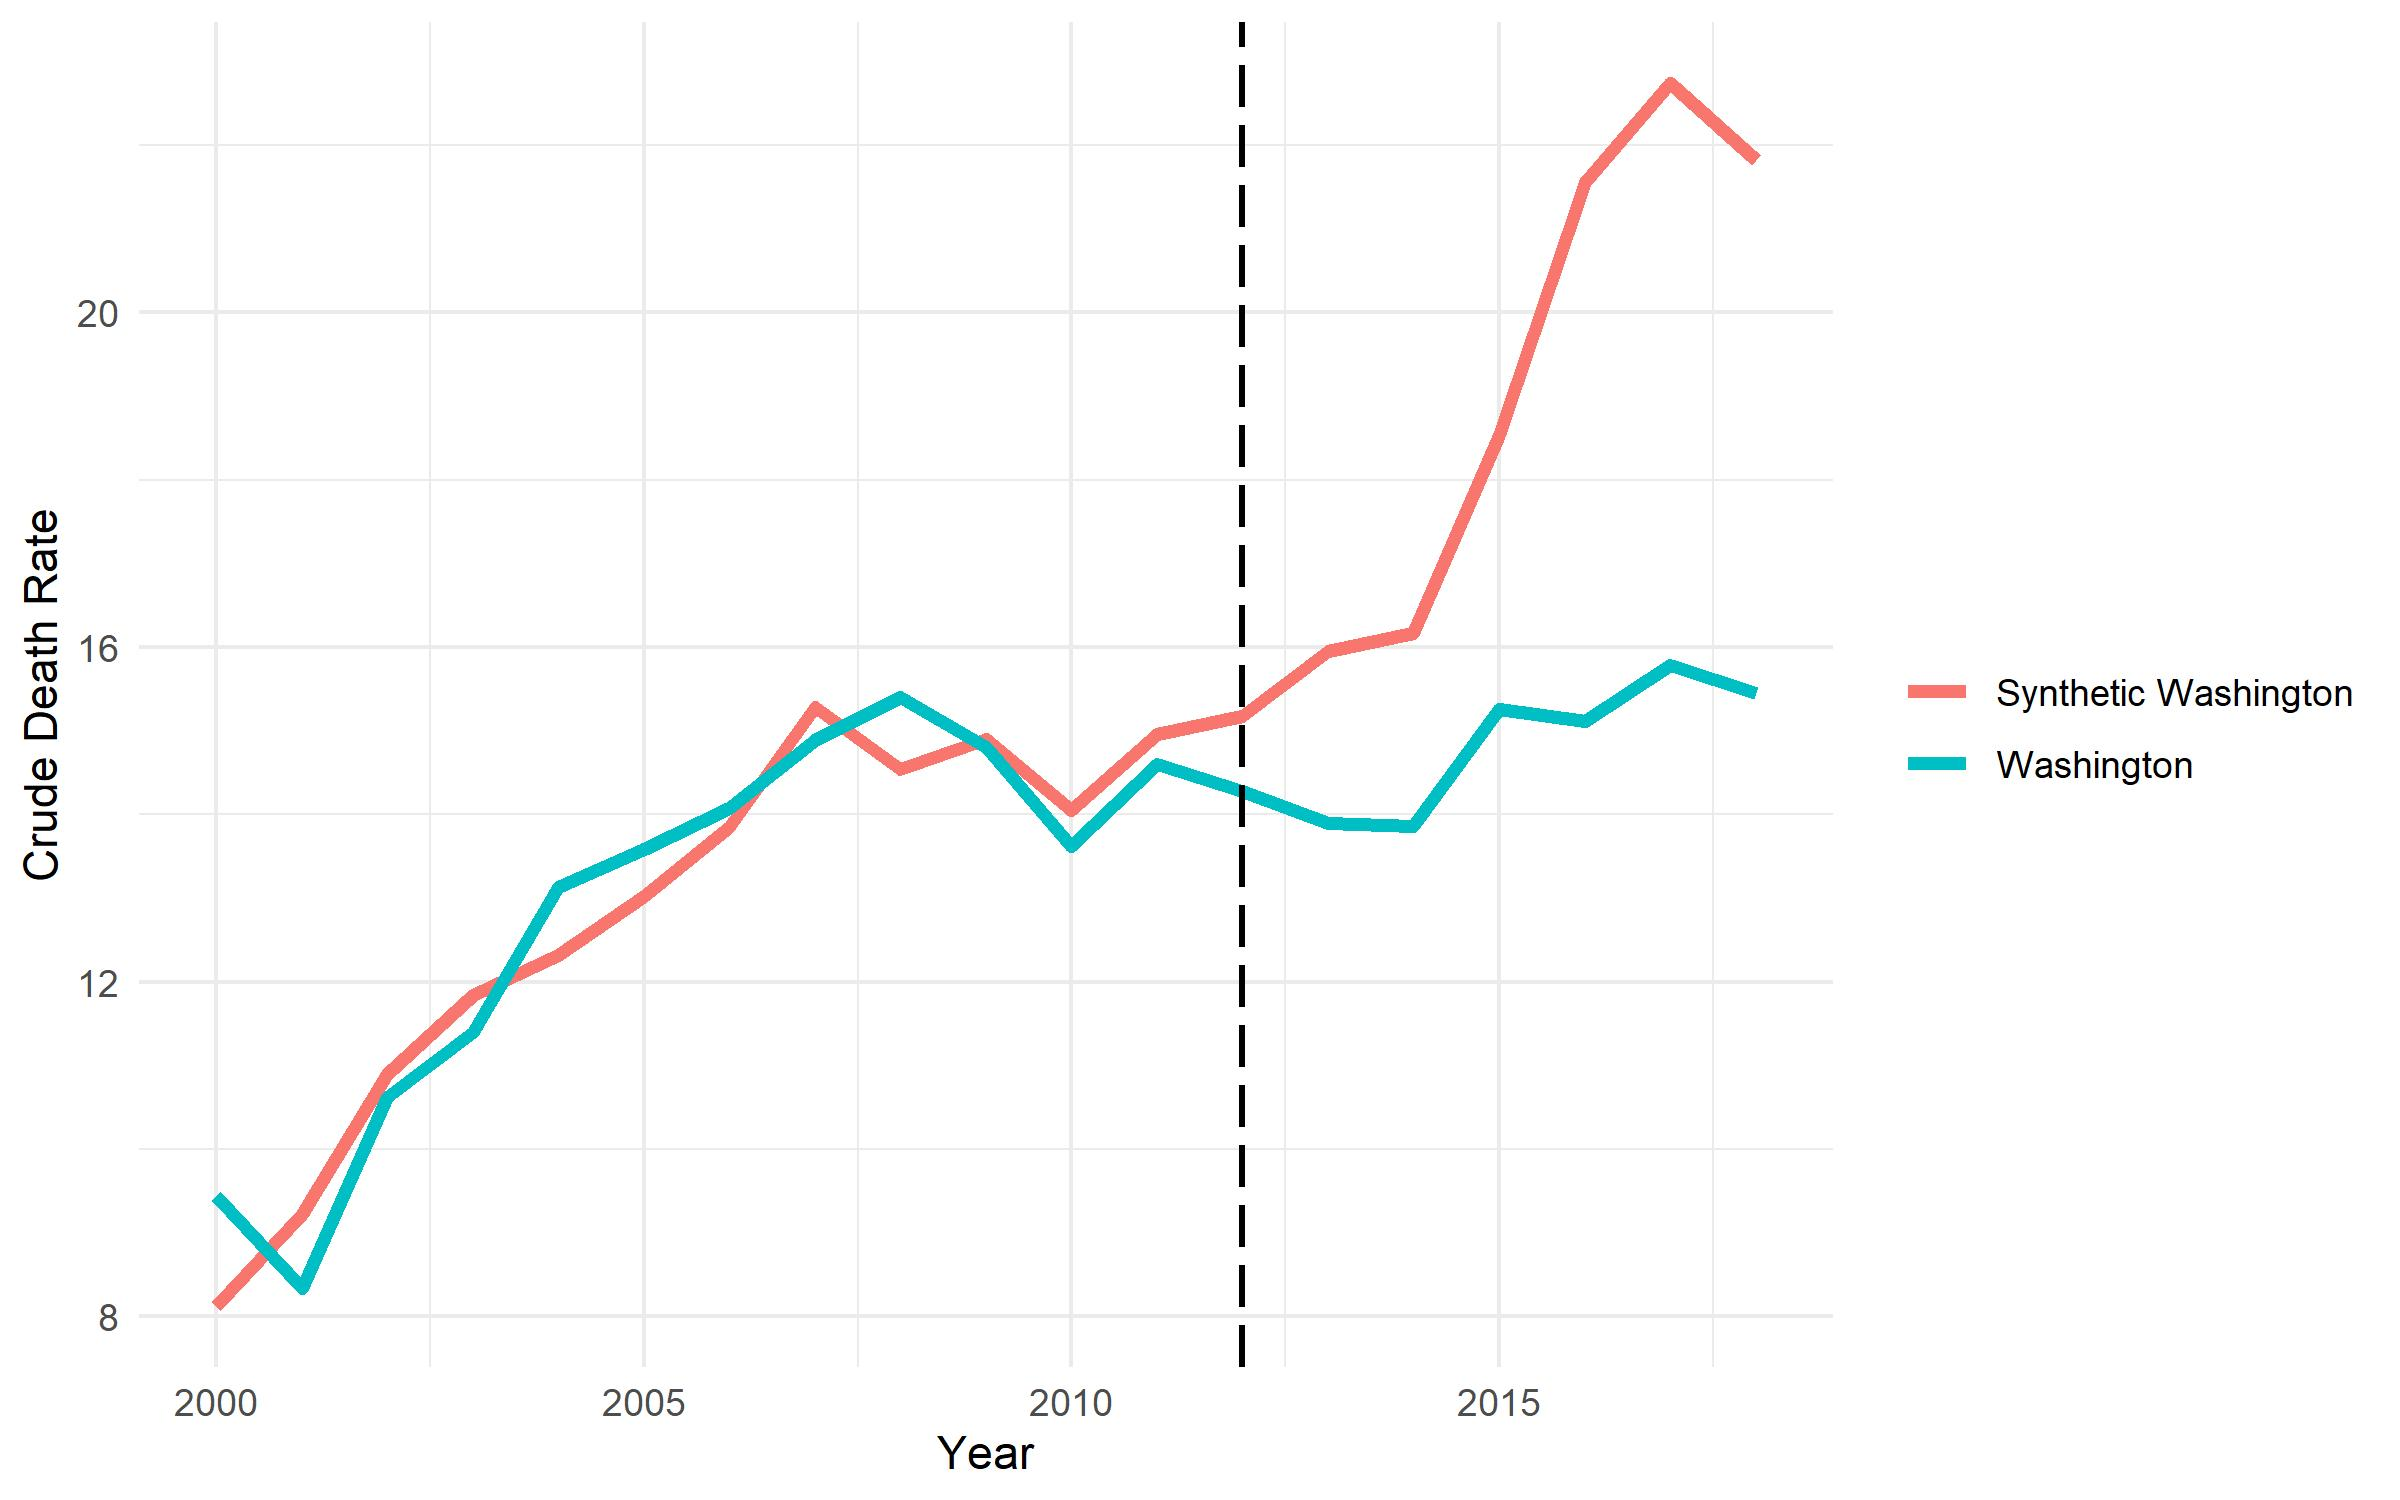
\includegraphics[width=0.85\textwidth]{trends_plot_washington}
	\end{center}
	\caption{Trends in Crude Death Rate: Colorado vs. Synthetic Washington}
	\label{fig:trends_plot_washington}
\end{figure}

\begin{figure}[H]
	\begin{center}
		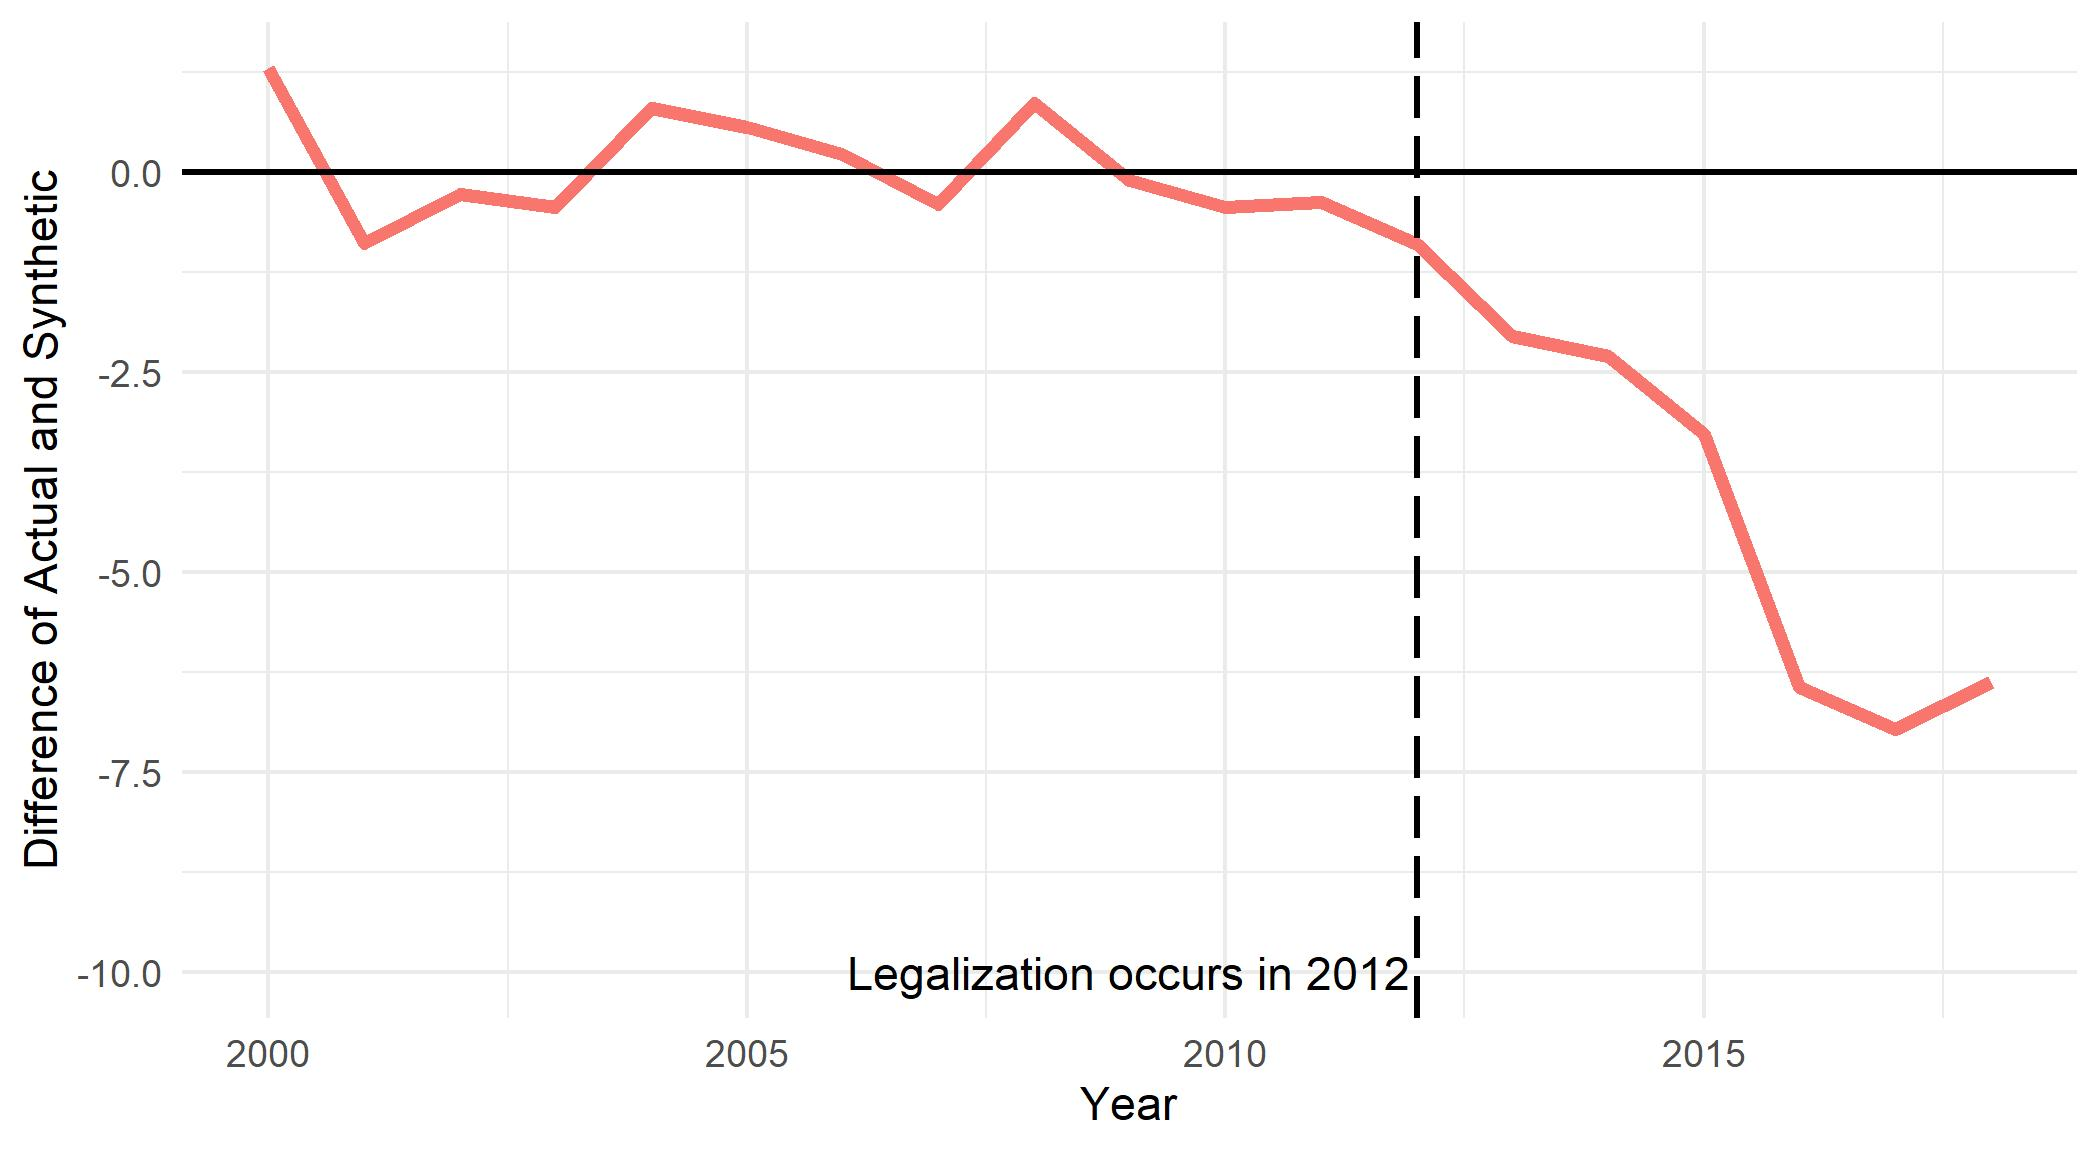
\includegraphics[width=0.85\textwidth]{diffs_plot_washington}
	\end{center}
	\caption{Differences in Crude Death Rate}
	\label{fig:diffs_plot_washington}
\end{figure}

\begin{table}[H]

\caption{\label{tab:causal_est_table_washington}Estimated Impact of Legalization on 
                         Drug Poisoning Death Rate: Washington}
\centering
\begin{tabular}[t]{>{\raggedleft\arraybackslash}p{1in}>{\raggedleft\arraybackslash}p{1in}>{\raggedleft\arraybackslash}p{1in}>{\raggedleft\arraybackslash}p{1in}}
\toprule
\multicolumn{1}{c}{} & \multicolumn{3}{c}{Drug Poisoning Death Rate} \\
\cmidrule(l{3pt}r{3pt}){2-4}
Years After Legalization & Actual & Synthetic & Estimated Causal Effect\\
\midrule
\cellcolor{gray!6}{2} & \cellcolor{gray!6}{13.864} & \cellcolor{gray!6}{16.167} & \cellcolor{gray!6}{-2.303}\\
4 & 15.121 & 21.554 & -6.433\\
\cellcolor{gray!6}{6} & \cellcolor{gray!6}{15.447} & \cellcolor{gray!6}{21.819} & \cellcolor{gray!6}{-6.372}\\
\bottomrule
\end{tabular}
\end{table}


\begin{figure}[H]
	\begin{center}
		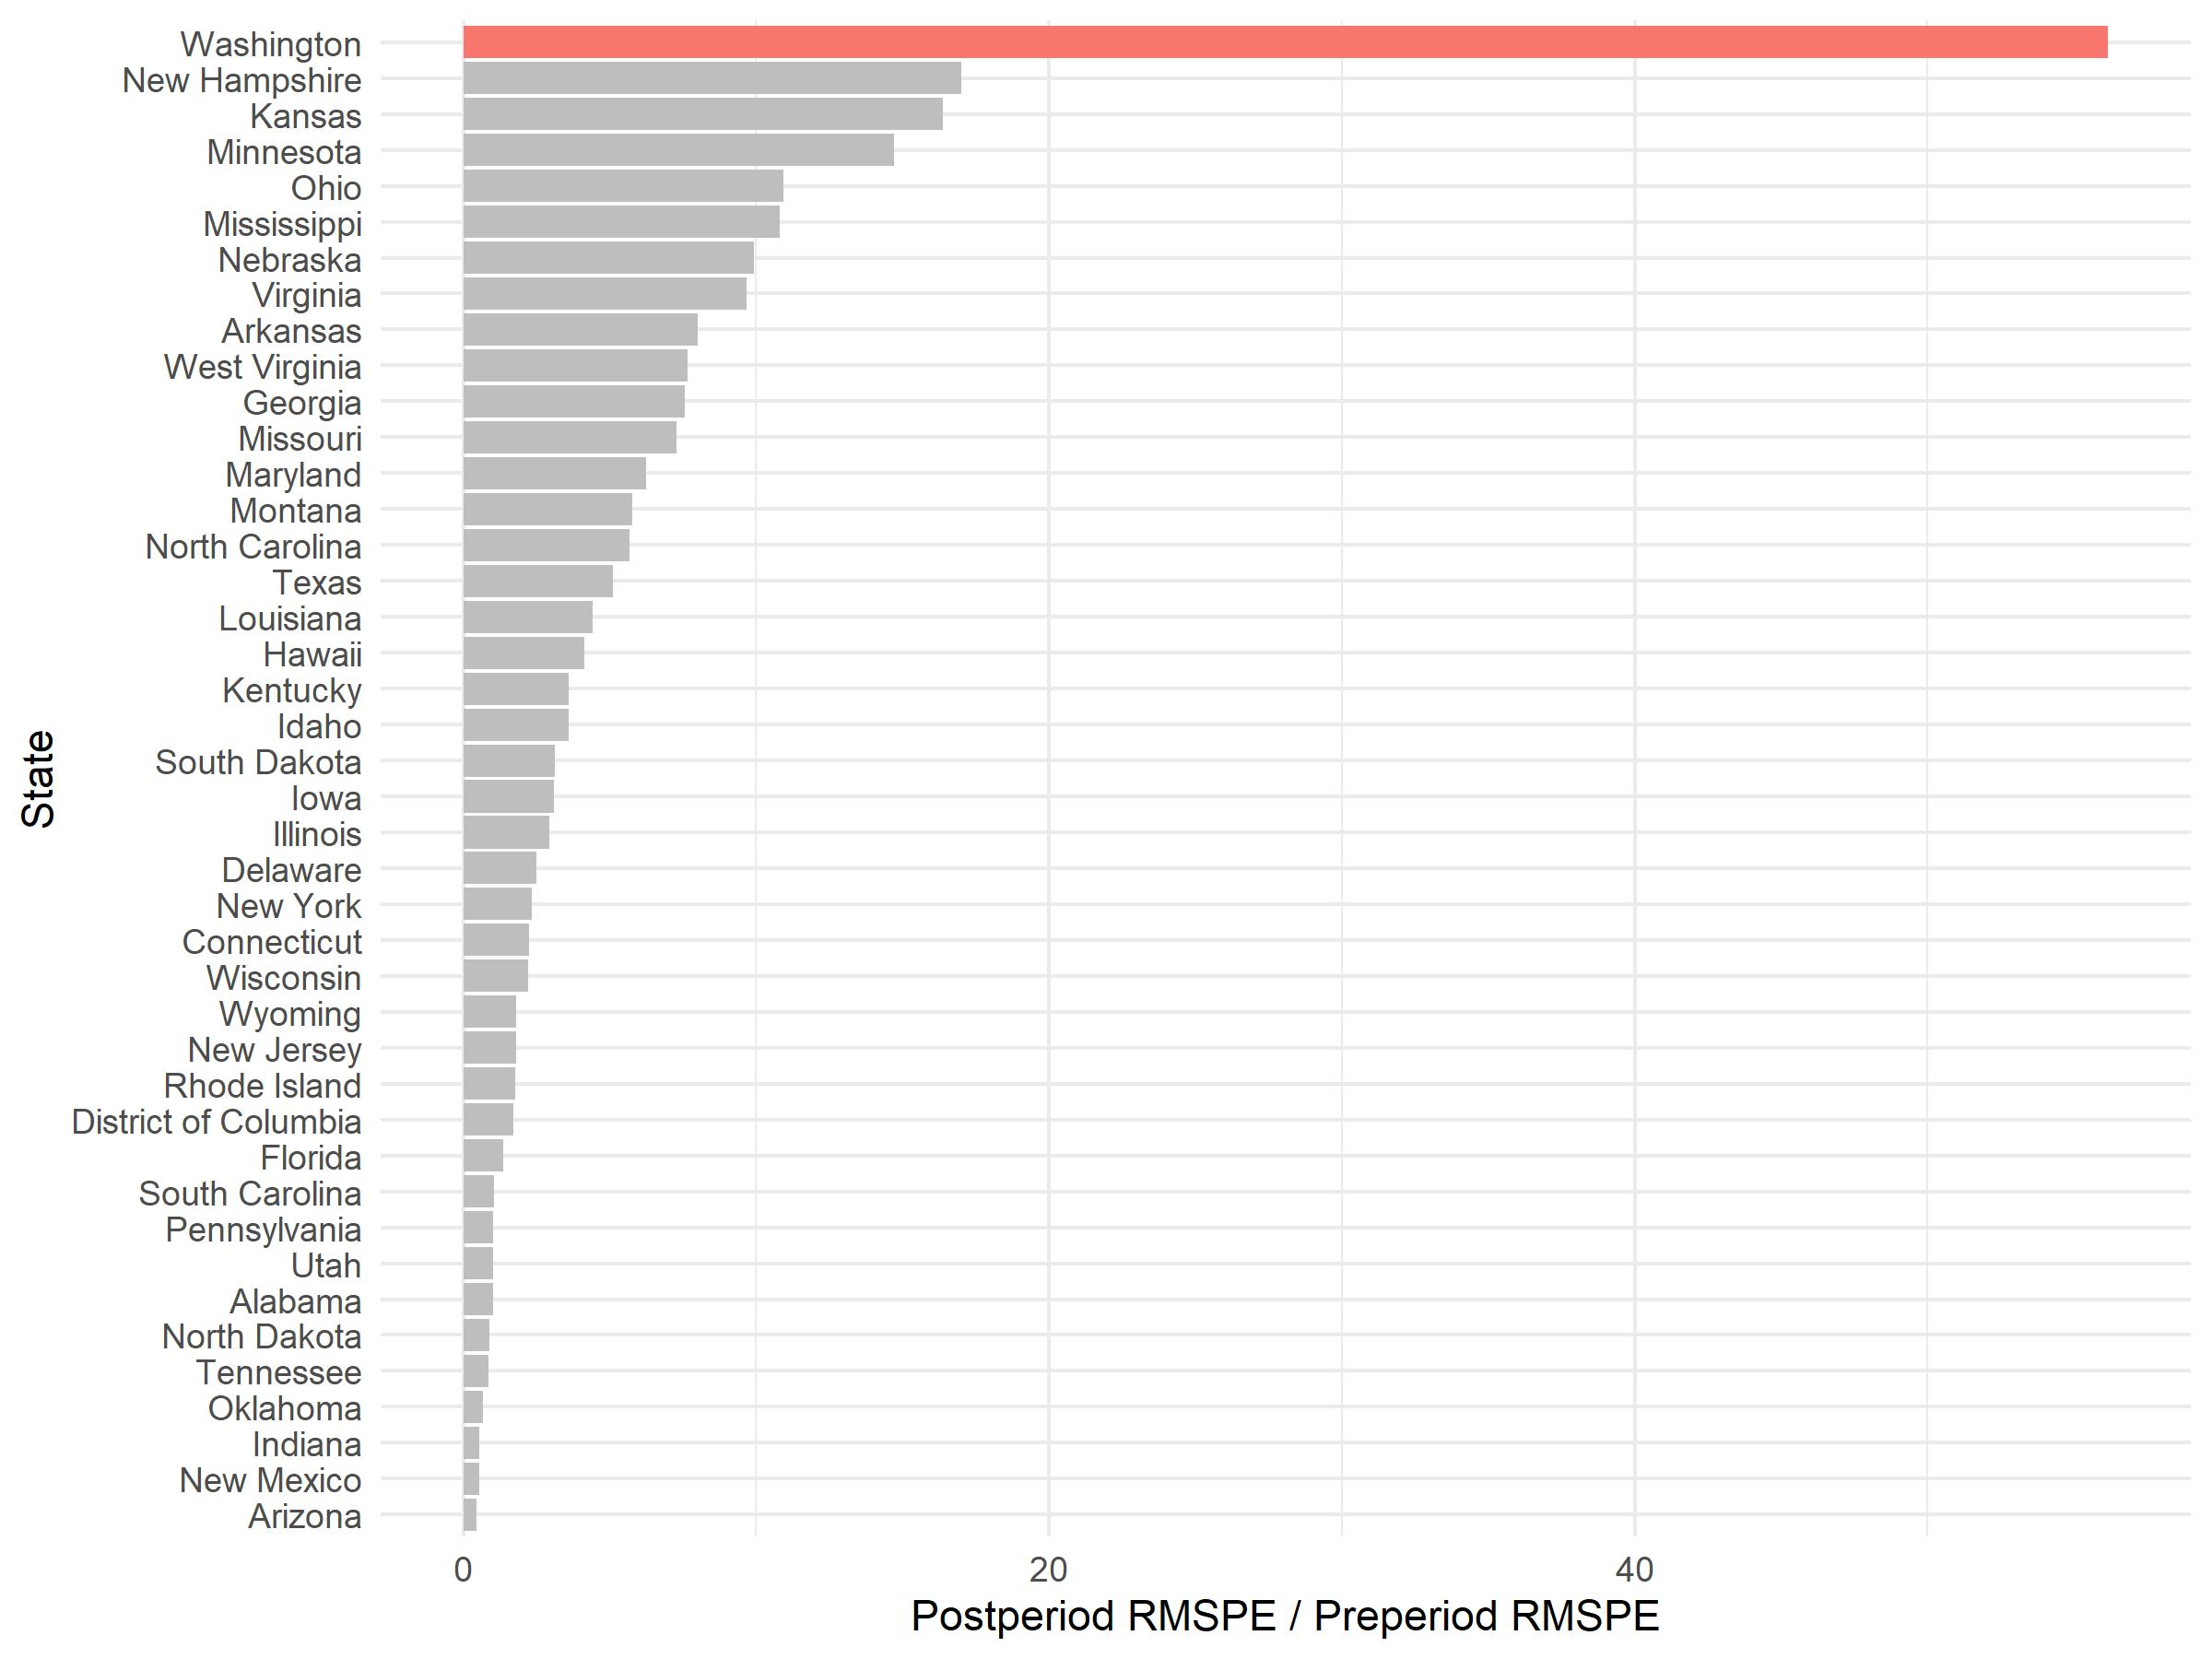
\includegraphics[width=0.85\textwidth]{mspe_plot_washington}
	\end{center}
	\caption{MSPE Ratio Plot}
	\label{fig:mspe_plot_washington}
\end{figure}

\begin{figure}[H]
	\begin{center}
		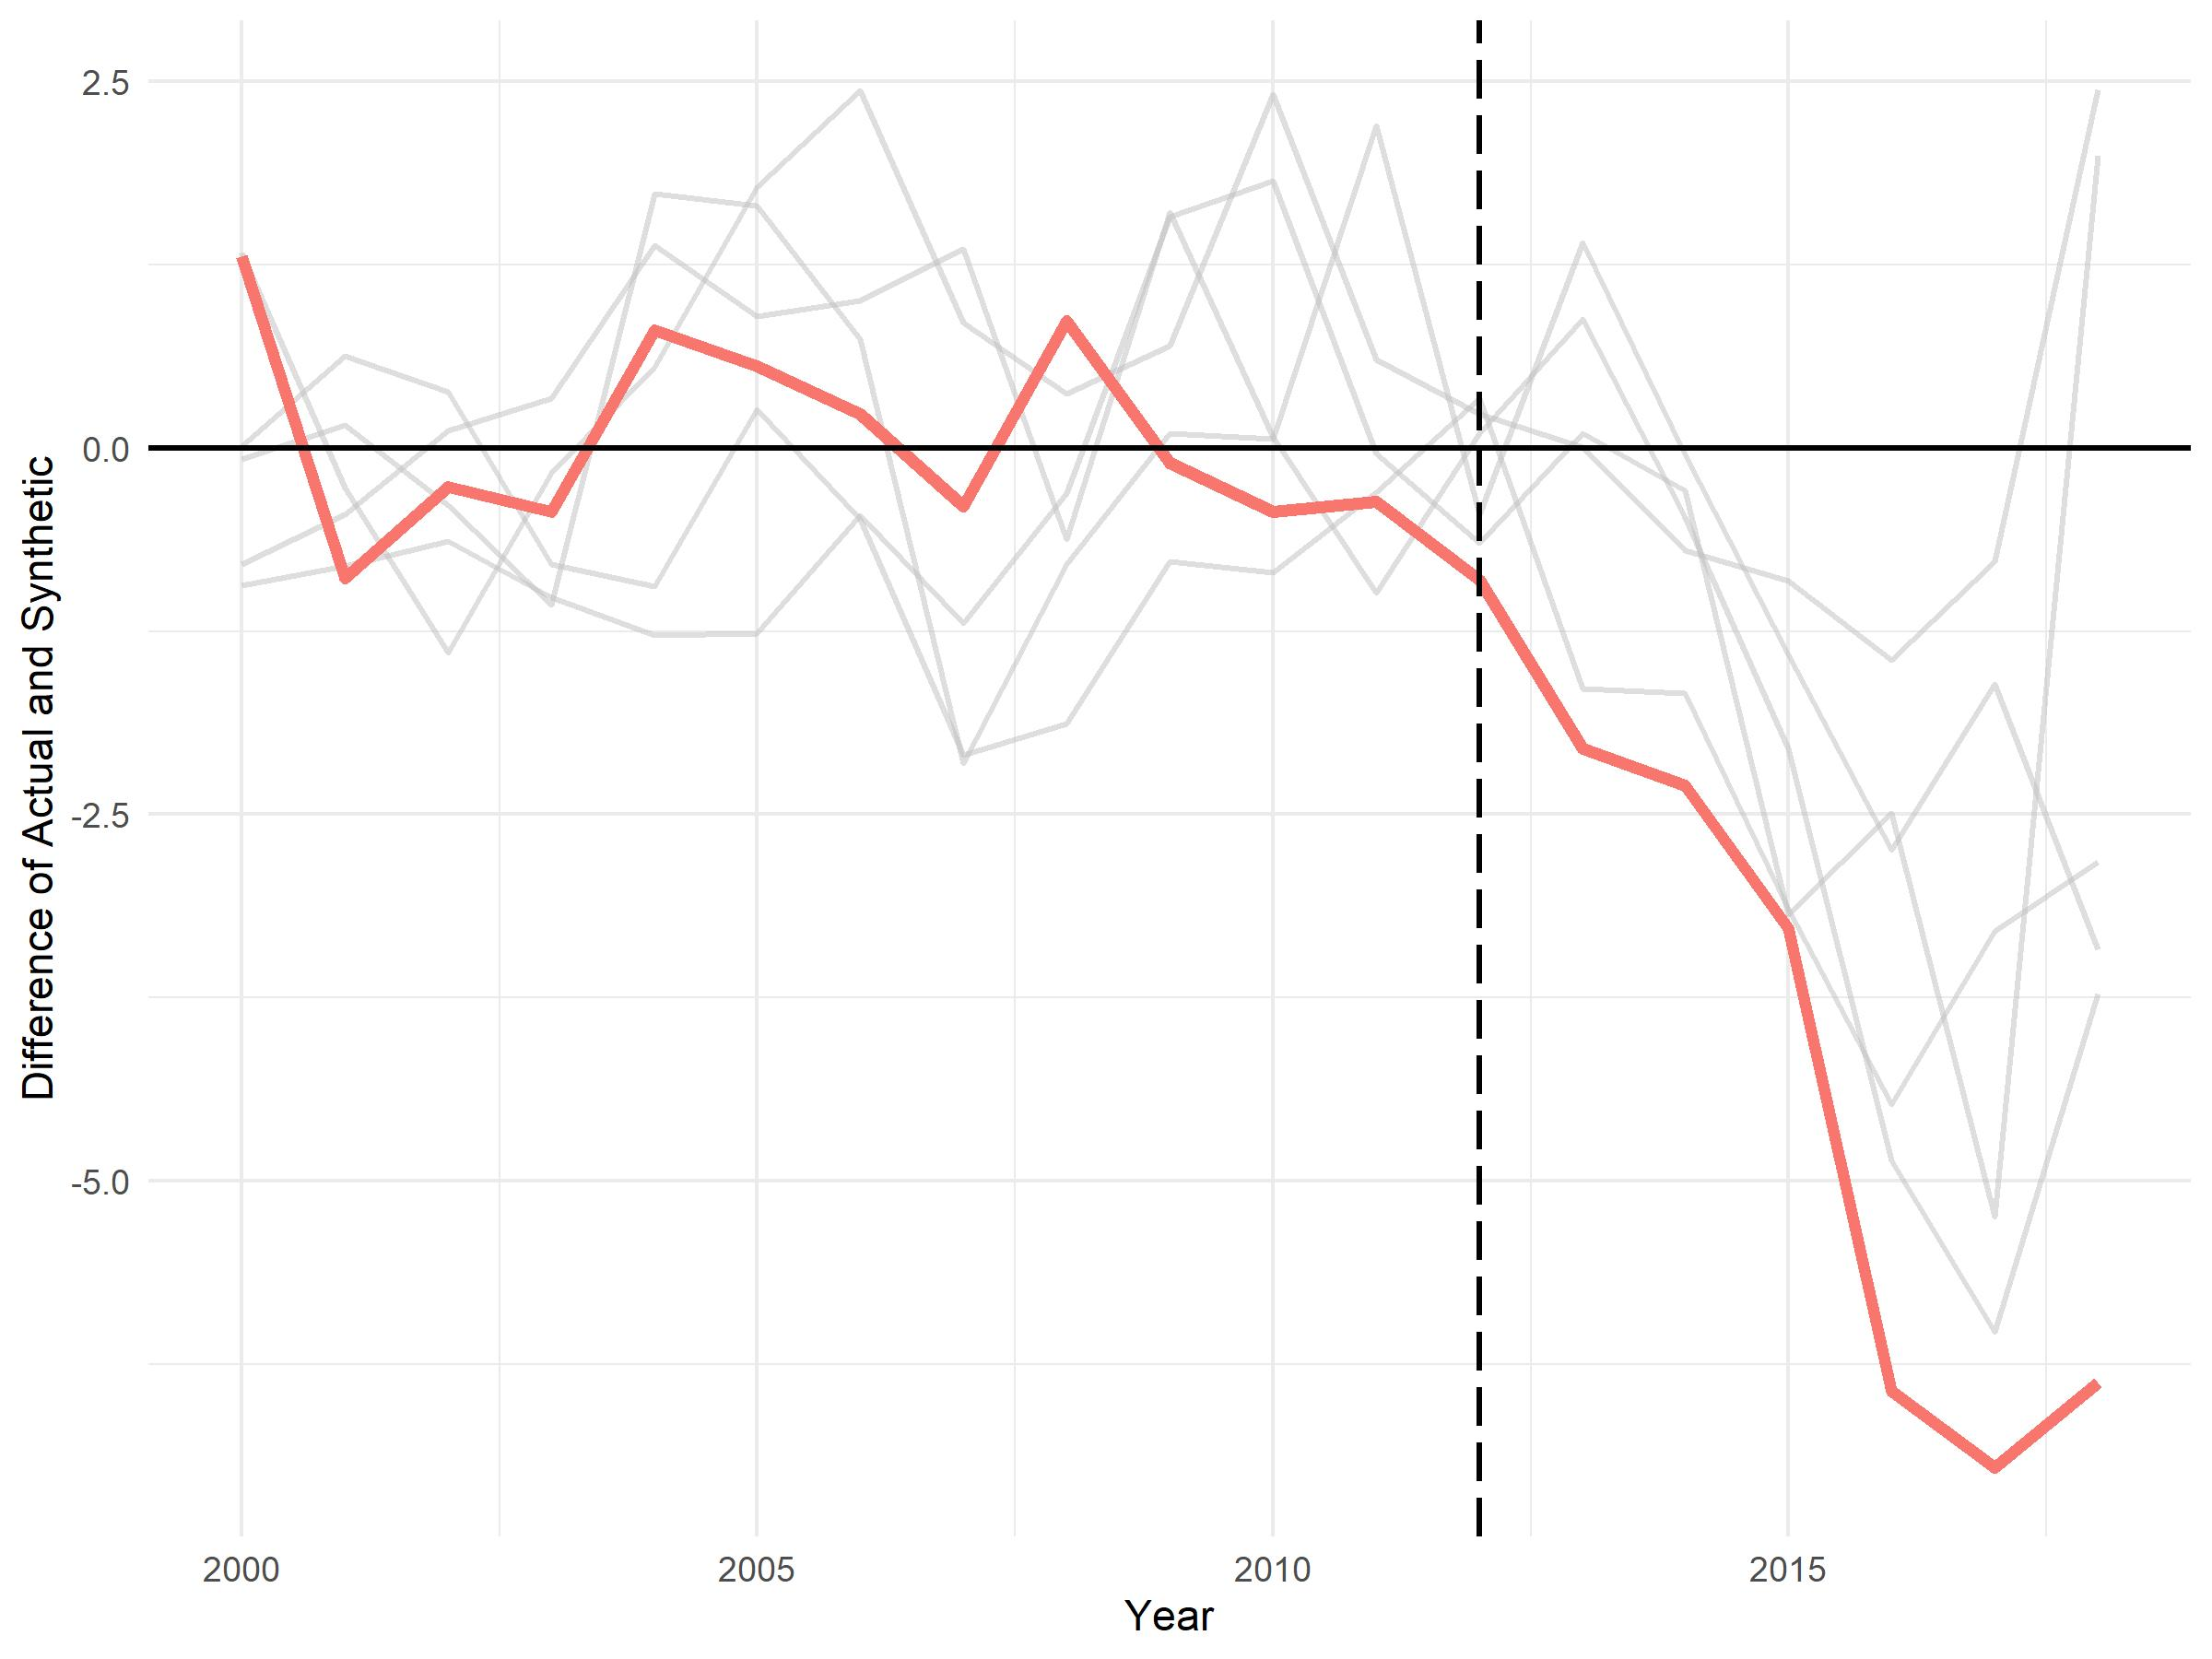
\includegraphics[width=0.85\textwidth]{placebos_plot_washington}
	\end{center}
	\caption{Placebos Plot}
	\label{fig:placebos_plot_washington}
\end{figure}


\end{document}

